\documentclass[letter, 11pt]{article}
\usepackage[utf8]{inputenc}
\usepackage{amsmath}
\usepackage{amsfonts,txfonts}
\usepackage{mathrsfs}
\usepackage[colorlinks, urlcolor=blue]{hyperref}
\usepackage{fourier}
\usepackage[top = 2.5cm, bottom = 2cm, left = 2cm, right = 2cm]{geometry}
\usepackage{graphicx}
\usepackage{scalerel,stackengine}
\usepackage{indentfirst}


\title{\textsc{Wavelet Clumps Project} \\
    \textsc{INF491: Astroinformatics}}

\author{Martín Villanueva}
\date{1 August 2016}

\begin{document}
\maketitle


\section{\textsc{Introduction}}

In this paper, we make an implementation and a theoretical/experimental study of the properties of multiresolution analysis with wavelets, in order to determine the hierarchical relations between clumps at different levels of details.

The innovative aspects of this work, come from performing wavelet decomposition and reconstruction directly over 3D data cubes, similar to approaches used on magnetic resonance imaging. Additionally, the implemented framework has out of the box tools to visualize the hierarchical relations between clumps, with tree structures and 3D visualizations of the results.

In section \ref{definition} a formal description of the problem to be faced is presented, section \ref{soa} introduces state of the art algorithms for clump identification and hierarchical relations, section \ref{proposal} gives an explanation of the proposed solution, section \ref{experiments} presents the experiments and analysis of the results obtained, and section \ref{conclusion} concludes.


\section{\textsc{Formal Problem Definition}} \label{definition}

In concise words the problem to be addressed consists on building an algorithm that automatically can identify clump structures, given a 3D spectroscopic cube of data (mostly from observations of cold molecular clouds) and determine the hierarchical relationships between them.\\

So in order to see the difficulties of the problem, it's imperative to understand what a clump is. There is some debate about the true nature of clumps, but is generally understood that a clump is an area of high density within a larger area of lower density, in relation to the star formation in molecular clouds \cite{Kennicutt}. This molecular clouds are usually non homogeneous in their density, and are composed of cores of high density gas matter contained and separated by low density areas. Each observation of such clouds, may contain multiple source cores in a very complex configurations. At the beginning astronomers analyzed these images manually (by eye), but this is no longer possible because of three major reasons:
\begin{enumerate}
    \item These manual methods doesn't scale as fast as the generation of new data observations, such as those performed by ALMA.
    \item The size of the images is huge and could contain hundreds/thousands of cores (Figure \ref{fig:barnard68}). So it may require a lot of time to analyze it manually.
    \item The results of clump identification performed (manually) by astronomers usually didn't match, because they have different conceptions and notions of what clumps are and how they relate each other.
\end{enumerate}

\begin{figure}[htpb!]
\centering
\includegraphics[width=6cm]{barnard68}
\caption{Barnard 68 molecular cloud}
\label{fig:barnard68}
\end{figure}

The third reason is the most important. As the image becomes more crowded with clumps, problems like blended emissions arise, where multiple dense cores converge in a nearby area. In these cases subjective biases become more evident as each astronomer might perceive the data differently. So the solution it to build an automated clump detection algorithm, removing individual biases and provide consistent and objective results.\\

Other complications are that 3D spectroscopic cubes (in FITS format) will be used instead of 2D cubes. They have \textit{right ascension}, \textit{declination} and \textit{frequency} coordinates with the associated observed intensity. Unlike the 2D version of collapsed cubes (in frequency), it is hard to analyze this kind of data by eye because of the extra dimension.\\

The final challenge is to determine the hierarchical relationships between the found clumps. As explained above, each dense core is often contained on lower density cores, constituting a hierarchical structure. Determining these relations is fundamental to understand processes like the \textit{star formation} \cite{Alves}.

    



\newpage
\section{\textsc{State of the Art}} \label{soa}

The problems stated in the previous section have been addressed during the last two/three decades using different approaches. Moreover, some of these have solved just a piece of the whole problem. In the following sections, a description its given about the principal algorithms used to solve the problems of \textit{clump identification} and determining the \textit{hierarchical relations}.

\subsection{\textsc{Clump Identification}} \label{clumping}

\begin{description}
    \item[\textbf{GaussClumps.}] This algorithm was proposed by Stutzki et al. \cite{Stutzki}, and was the first successful approach to handle the problem of automatically detecting clumps. The main idea is to adjust Gaussian profiles that best fits each of the emission peaks. There are two reasons to use Gaussian functions over some other choice: 1) The experimental observations of the most abundant molecules on molecular clouds, have shown that his intensity distribution have a shape more or less like Gaussians. 2) The \textit{redshift}  phenomenon due to the relative movement of the observed structures, produces gaussian shaped frequency distributions.

    The algorithm iteratively searches for the current emission peak, and tries to fit a Gaussian function (searching for the best parameters of that Gaussian) through a minimization process. Then this Gaussian is subtracted from the data cube, and the same step is repeated over the residual cube. As result we get a set a gaussians with different positions, orientations and intensities. The sum of all this Gaussian components plus the background noise, allows us to reconstruct the data cube.

    In this algorithm each Gaussian is considered as a single clump, and because Gaussians could overlap between them, then it is possible that pixels are assigned to more than one clump.


    \item[\textbf{ClumpFind.}] This algorithm was developed by Williams et al. \cite{Williams}.  It was motivated by how the human eyes identify structures on images, i.e, how the eye decomposes the maps into clumps by looking at the contour levels in a gradually and decreasing way. So the algorithm works by contouring the data at multiples of the RMS noise of the observations. It starts from the highest level, where isolate cores are identified and each of these are considered as a new clump. Then this step is repeated by gradually decreasing the level where to contour,  identifying isolate structures and connecting them with clumps identified at higher levels, or defining them as new clumps otherwise. When a clump identified at a given level touches more than one clump identified at a previous level, then this structure correspond to a blended emission, and should be splitted. To do that a \textit{friends-of-friends} strategy is used, assigning each pixel of the identified structure to one of the adjoining clumps (\textit{with more friends}).

    As result of this process a \textit{Clump Assignment Array} structure is generated, where each pixel is assigned exclusively to one clump, as shown in Figure \ref{fig:cf}. A key characteristic of ClumpFind is that no a priori clump profile is assumed, and then the identified clumps can have any shape.
    \begin{figure}[htpb!]
    \centering
    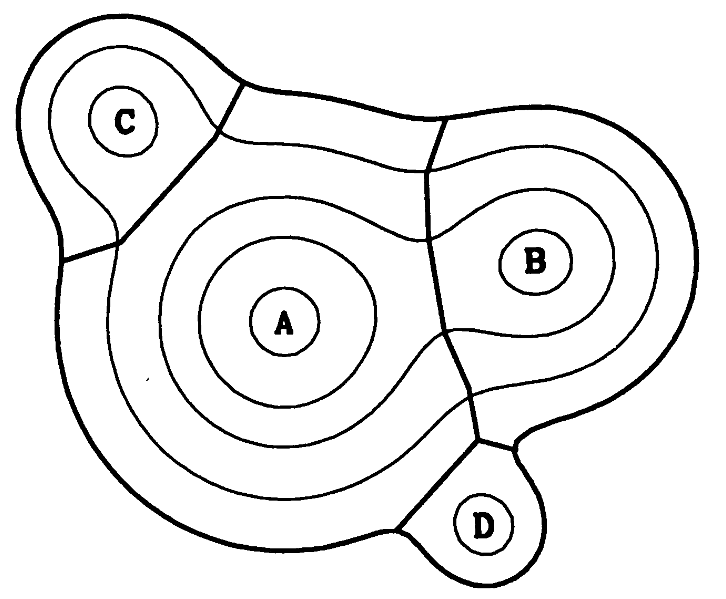
\includegraphics[width=8cm]{cf}
    \caption{ClumpFind results on 2D data (Source: \cite{Williams})}
    \label{fig:cf}
    \end{figure}

    \item[\textbf{FellWalker.}] A different approach was proposed recently by Berry \cite{Berry}, in which a gradient-tracing scheme similar to \textit{hill-climbing} it is used in order to reach a local emission peak, which defines a new clump. FellWalker like ClumpFind, segments the supplied data cube into a number of disjoint regions, each associated with a single significant peak.

    The algorithms works by computing ascent paths (with the highest gradient) for each single pixel (Figure \ref{fig:fw}). These paths have two alternatives: 1) To reach a local peak and therefore finding a new clump. In that case a new search it's performed on a wider neighborhood to verify that it is really a peak. 2) Reach another ascent path computed previously, and assign the pixels on the path to the corresponding (crashed) clump. At the end of the algorithm, detected clumps with low dip between them, are merged as a single clump.
    \begin{figure}[htpb!]
    \centering
    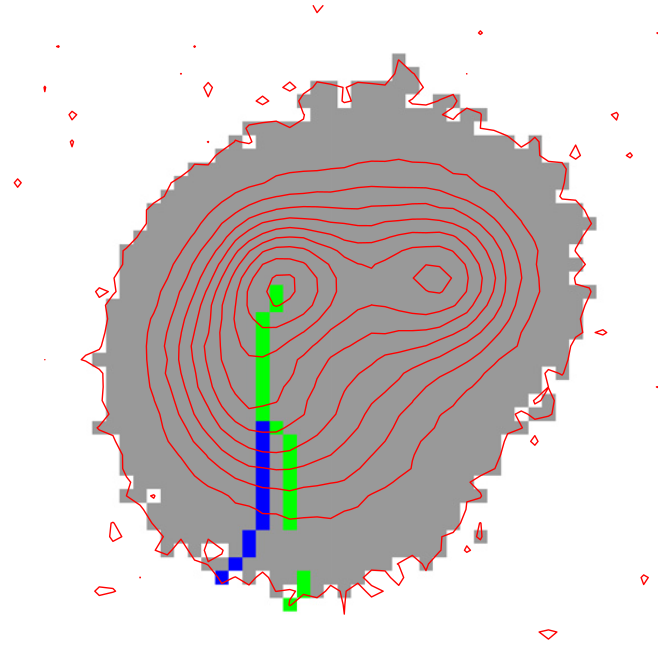
\includegraphics[width=8cm]{fw}
    \caption{Two ascent paths of FellWalker on 2D data (Source: \cite{Berry})}
    \label{fig:fw}
    \end{figure}

\end{description}


\subsection{\textsc{Hierarchical Relations}}

\begin{description}
    \item[\textsc{Dendrograms.}] Dendrograms approach was proposed by Rosolowsky et al. \cite{Rosolowsky}. This method is conceptually different from local segmentation algorithms like ClumpFind or FellWalker, since it aims to track the hierarchical structure over a range of scales. Similar to ClumpFind, this algorithm computes the \textit{isosurfaces} (surfaces with the same intensity) for molecular data cubes, representing the hierarchical structure of these, in a tree data-structure also know as Dendrograms. Points in the dendrogram structure correspond to specific volumes in data cubes, defined by their bounding isosurfaces.

    If the ClumpFind algorithm divides a contour map in pieces of a puzzle, then the Dendrograms try to divide that puzzle in a collection of different layers that represents the cores. The order and structure of the tree, defines the physical relations between the identified cores.

    \item[\textsc{Multiresolution Analysis.}] Multiresolution Analysis (MRA) it is a technique widely used in the last years to analyze astronomical data images. In particular one of the major tools to perform MRA is the Wavelet Transform, which maps input data to the \textit{scale-position} Wavelet space. As explained by Starck \cite{Starck}, \textit{Discrete Wavelet Transform} (DWT) can be used to transform the data and see it with different resolutions, i.e, have a view of the data with different levels of details, and then we can see fine-grained to coarse-grained details. A not so useful type of DWT is the \textit{Stationary Wavelet Transform} (SWT), also called \textit{À trous} wavelet transform. This consist on a redundant version of DWT, that has the property of mapping input images to images in the wavelet space with the same size (because of the redundancy). Because of that, all the analysis could be done at the Wavelet space.

    In his study of the stellar \textit{Initial Mass Function} (IMF), Alves et al. \cite{Alves} applied the SWT to images of interstellar molecular clouds, in order to have a detailed knowledge of the spectrum of masses of dense cores. The clump identification procedure first maps the corresponding (2D) image, to the wavelet space at different scales. For a given scale $i$, structures are isolated at $3\sigma_i$, with $\sigma_i$ being the noise of the image at scale $i$. Then a detected structure at scale $i$ is connected with a structure at scale $i+1$ if its local maxima drops in the structure at scale $i+1$.

    On the other side Gregorio et al. \cite{Gregorio} follows a very similar approach, performing SWT over 2D images to get a multiresolution view of the data. However he wasn't satisfied with the thresholding step of above, arguing that  simple thresholding isn't the best way of segmenting astronomical data. Instead he proposed to use clump identification algorithms (like ClumpFind), to segment the data at the different levels on the Wavelet space. A graphical sample of this results are shown in Figure \ref{fig:greg}.
    \begin{figure}[htpb!]
    \centering
    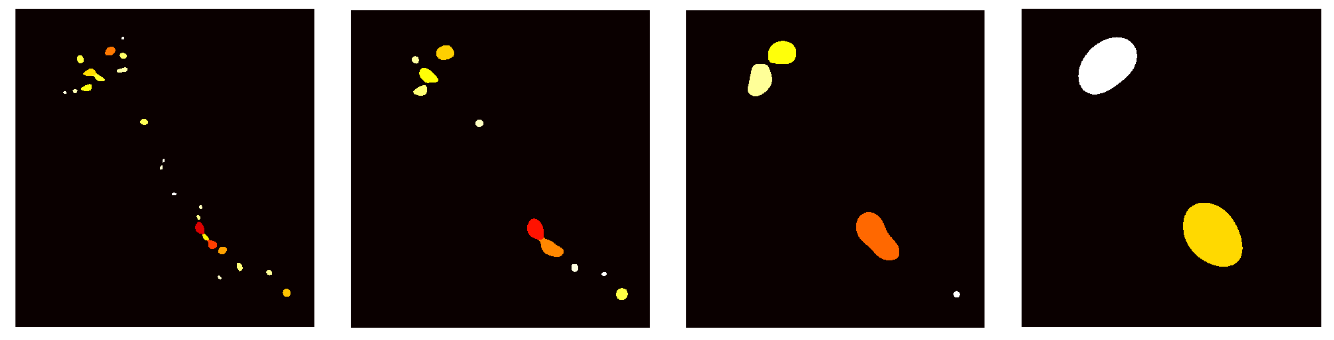
\includegraphics[width=14cm]{greg}
    \caption{Clump Identification at 4 different scales on Wavelet Space (Source: \cite{Gregorio})}
    \label{fig:greg}
    \end{figure}
    Applying the same criterions as Alves \cite{Alves}, a hierarchical relation could be stated between the structures found at the different scales, to create a Dendrogram like structure.
\end{description}



\newpage
\section{\textsc{Proposed Solution}} \label{proposal}

In order to solve the problem of identification and hierarchical relations of clumps on spectroscopic data cubes, we propose to extend the ideas of Alves \cite{Alves} and Gregorio \cite{Gregorio}, to 3D data cubes. Then a MRA will be required over the 3D data cube, i.e, a 3D discrete Wavelet transform should be applied to extract the features at different scales. After computing the 3D DWT, the procedure continues similarly to the former; A clump identification/segmentation algorithm is applied to each new cube, and then the results of the different levels are summarized in a Dendrogram tree structure. An outline of this procedure is shown on Figure \ref{fig:wavclump}.
\begin{figure}[htpb!]
\centering
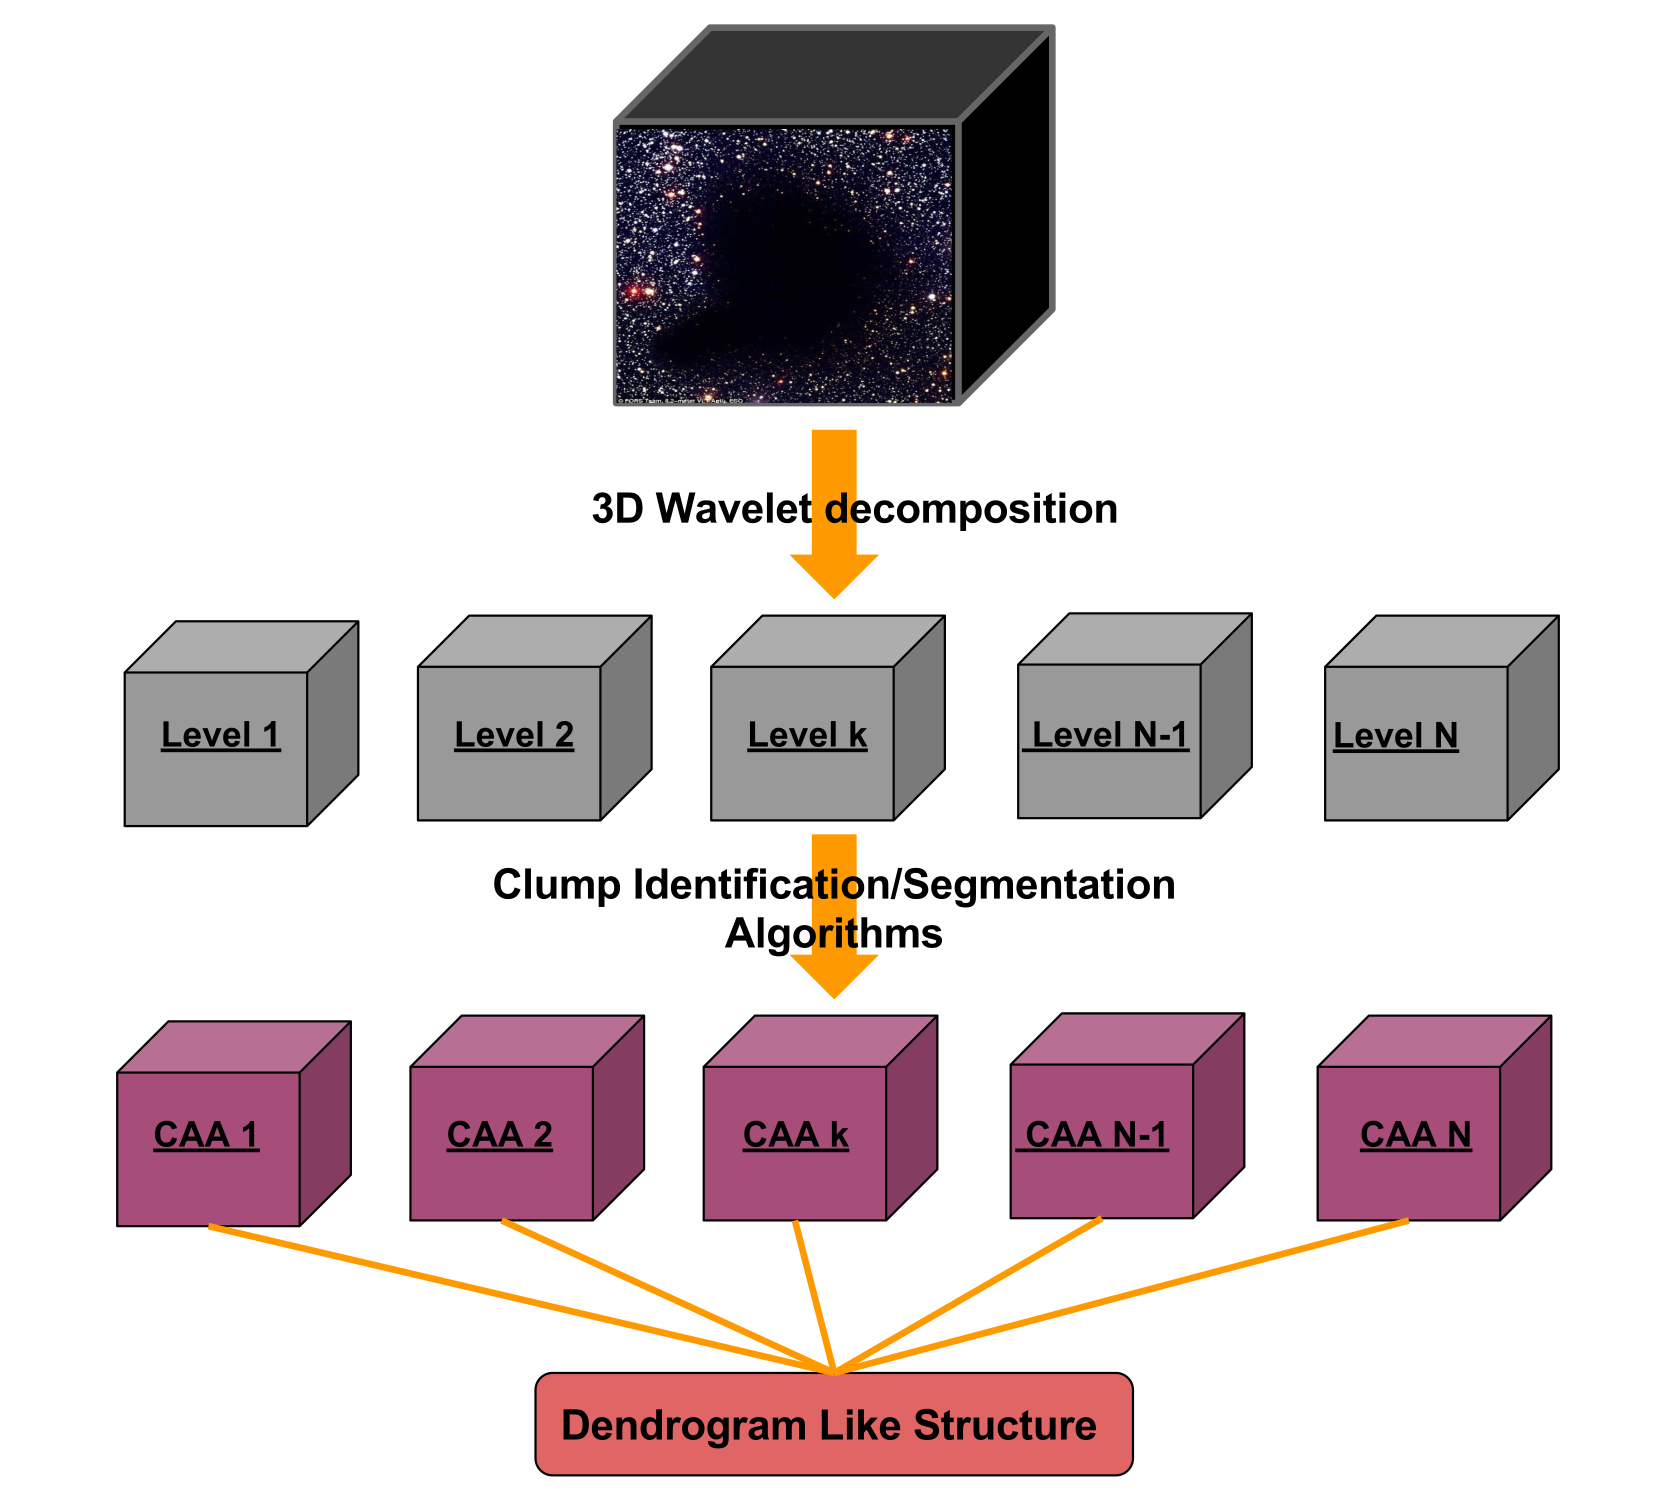
\includegraphics[width=12cm]{wavclump}
\caption{Proposed Solution Outline}
\label{fig:wavclump}
\end{figure}
However, some considerations must be taken into account:
\begin{enumerate}
    \item As explained before, the SWT maps input images to images in the Wavelet space with the same size. If we are working with dense 3D data cubes, the process of computing the SWT for each level will require a considerable computing time and memory space. Additionally, we did not find any off-the-shelf software package that implements the 3D version of the SWT.
    \item The standard DWT works on N-dimensional data, but it maps the input image to a sparse representation on the Wavelet space, which has incompatible dimensions with the former. An option is to compute the Inverse Discrete Wavelet Transform (IDWT) for each level, using those as the MRA representation.
    \item In order to get coherent results, an appropiate 3D wavelet has to be chosen (or constructed) such that the features computed at the different levels are meaningful.
\end{enumerate}

Additionally we propose to take an intermediate point between Alves and Gregorio Identification/Segmentation step. Images on a low level (in the Wavelet space) have fine-grained details, and so they need a robust algorithm to perform the segmentation step. On the other hand, images with a high level have coarse-grained details, and so they don't need a complex algorithm to segment it, probably with just a thresholding segmentation will be good enough. Therefore, it is possible to take the good things from both approaches. In thit way, the whole process could be optimized by performing robust (and computationally expensive) methods on data with fine-grained details, and performing some simpler methods (and computationally cheap) on data with coarse-grained details.

Fast segmentation can be done with several methods: Simple thresholding, adaptive thresholding, watershed algorithm, and many more from the computer vision and image processing fields.


\section{\textsc{Experiments and Results}} \label{experiments}

\begin{description}
    \item[\textsc{Experiment Settings.}] In the following experiments we are using a FITS image of Orion Methanol observations from the ALMA data science verification archive \footnotemark[1]. It consists of a cube with $40 \times 40$ pixels for spatial resolution, and $41$ channels of frequency.

    For the Wavelet MRA we test six different \textit{standard} wavelet families in order to compute the 3D DWT: \textit{Haar}, \textit{Daubechies}, \textit{Symlet}, \textit{Coiflet}, \textit{Biorthogonal} and \textit{Reverse Biorthogonal}. In each case the number of \textit{vanishing moments}  was set according to the MATLAB Wavelet Toolbox indications \footnotemark[2], plus experimental tuning.    

    To compute the clumps at each level of decomposition, we use the Fellwalker algorithm (see Section \ref{clumping}) implemented in ACALIB \footnotemark[3], with the default parameters of Starlink's CUPID software package \footnotemark[4].

    \footnotetext[1]{\href{http://jvo.nao.ac.jp/portal/alma/sv.do?action=dataset.info&datasetId=ALMA00000035}{Orion FITS} from ALMA data science verification at JVO.}
    \footnotetext[2]{\href{www.mathworks.com/help/wavelet/ug/wavelet-families-additional-discussion.html}{Matlab's Wavelets Families}.}
    \footnotetext[3]{\href{https://github.com/ChileanVirtualObservatory/ACALIB}{ACALIB's Github website}.}
    \footnotetext[4]{\href{https://github.com/Starlink/starlink/tree/master/applications/cupid}{CUPID's Github website}.}

    \item[\textsc{Concept Test.}]
     First, some tests are performed about the multiresolution representation of the data in order to visualize the effects of extracting the low frequency components of the signal. To visualize the results, four slices at $\text{frequencies }= \ 12,\ 18,\ 24,\ 30$ are shown (Figure \ref{fig:level0}).
    \begin{figure}[htpb!]
    \centering
    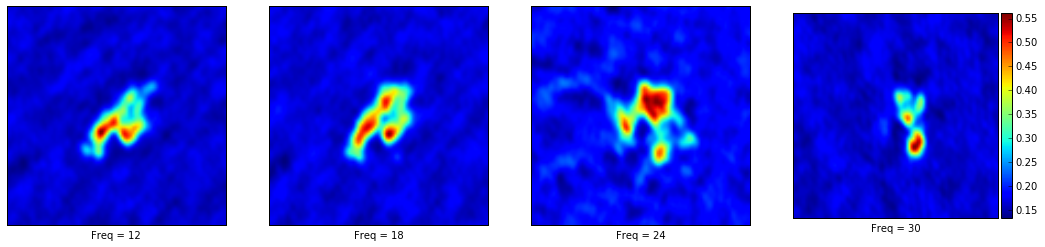
\includegraphics[width=15cm]{level0}
    \caption{Original data slices}
    \label{fig:level0}
    \end{figure}

    To perform the multiresolution analysis, a 3D DWT is used with a Daubechies wavelet (\texttt{db5}). The first four levels are obtained by sequentially computing the low-pass (approximation) coefficients, with the corresponding reconstruction process. The results of that reconstructions are shown in figures \ref{fig:level1} and \ref{fig:level3}, for the levels $1$ and $3$ respectively.

    \begin{figure}[htpb!]
    \centering
    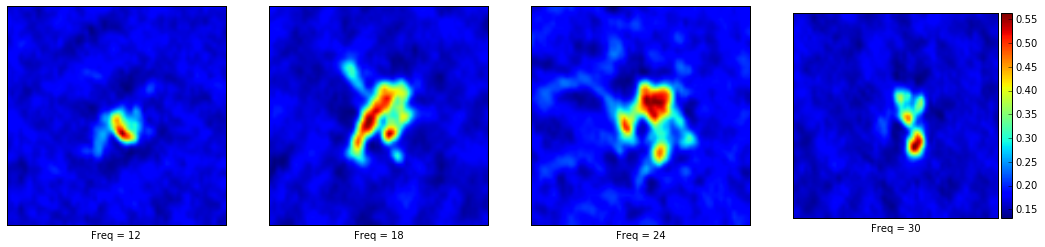
\includegraphics[width=15cm]{level1}
    \caption{Slices at level 1}
    \label{fig:level1}
    \end{figure}

    % \begin{figure}[htpb!]
    % \centering
    % 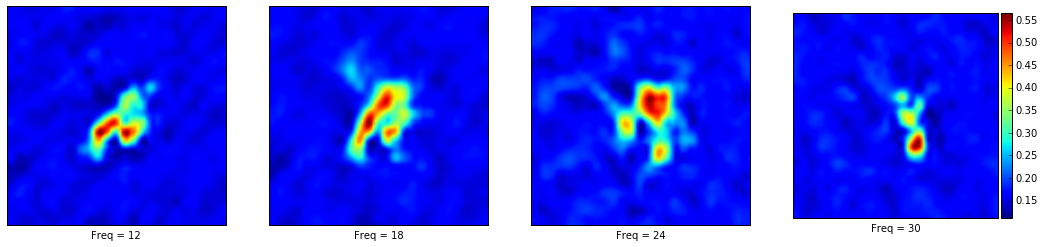
\includegraphics[width=15cm]{level2}
    % \caption{Slices at level 2}
    % \label{fig:level2}
    % \end{figure}

    \begin{figure}[htpb!]
    \centering
    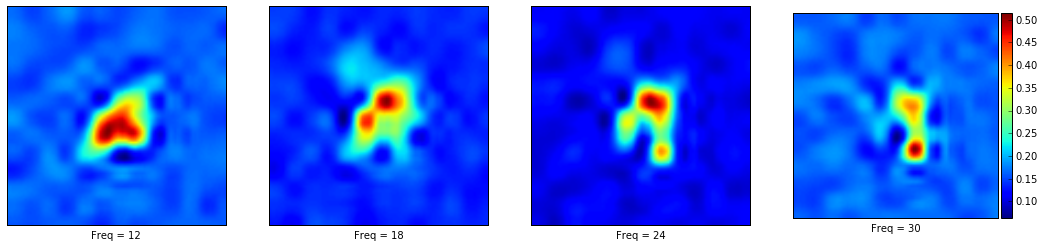
\includegraphics[width=15cm]{level3}
    \caption{Slices at level 3}
    \label{fig:level3}
    \end{figure}

    % \begin{figure}[htpb!]
    % \centering
    % 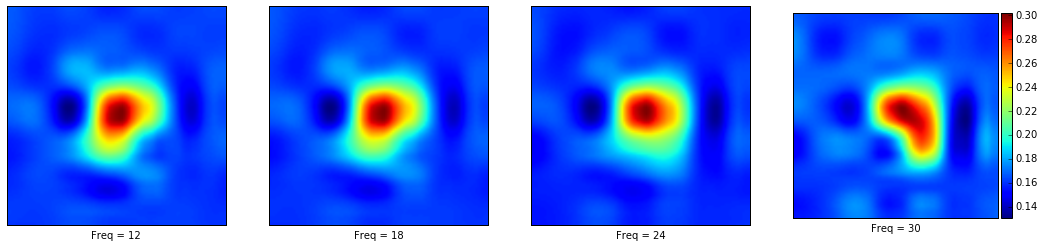
\includegraphics[width=15cm]{level4}
    % \caption{Slices at level 4}
    % \label{fig:level4}
    % \end{figure}

    It can be noted that as the level gets higher, less detailed data we get, i.e, the coarse-grained details are appearing. As stated in Section \ref{proposal}, it is clear that in the high levels the clump structures are much more easy to identify that the ones in lower levels.

    In order to verify the last point, a thresholding procedure similar to Alves \cite{Alves} was performed on data at level $1$ and $3$, which can be seen in Figures \ref{fig:th1} and \ref{fig:th3} respectively.
    \begin{figure}[htpb!]
    \centering
    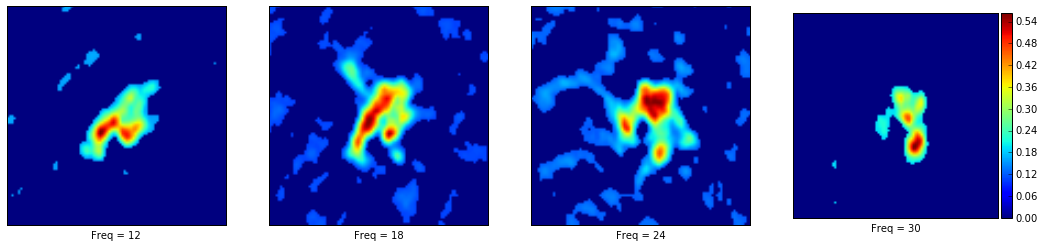
\includegraphics[width=14cm]{threshold1}
    \caption{Thresholding slices at level 1}
    \label{fig:th1}
    \end{figure}

    \begin{figure}[htpb!]
    \centering
    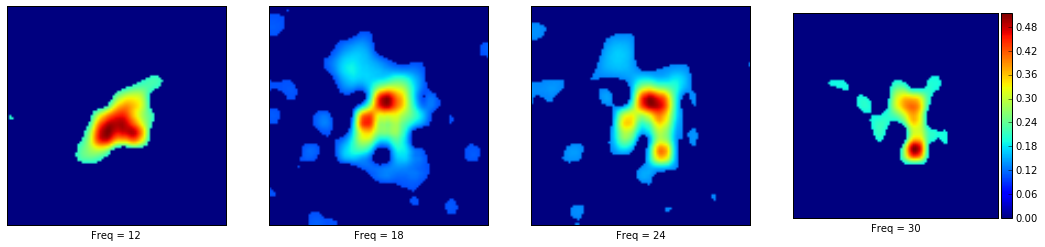
\includegraphics[width=14cm]{threshold2}
    \caption{Thresholding slices at level 3}
    \label{fig:th3}
    \end{figure}
    Thresholding the coarse-grained data gives very good results, getting almost the exact clump structure. On the other hand, thresholding the fine-grained data gives poor results, detecting regions that are not actually part of cores.


    \item[\textsc{Analysis of Decomposed Data.}]
    There is a main problem in the formulation of the proposed solution (Section \ref{proposal}): The two principal clumping algorithms (Fellwalker and Clumpfind) are very dependent of the RMS value of the data, in fact many of the other parameters are set as multiples of the RMS value. Therefore, if the RMS of approximated data change with the decomposition level, then the corresponding algorithm will change his behavior.

    In Figure \ref{fig:rms} we show the RMS change with the decomposition level for each wavelet. It is clear that there exist an inverse relation between them. This result makes total sense if we recall the MRA process: At each step $8$ approximation coefficients are computed ($\{ \text{LLL},\ \text{LLH},\ \text{LHL},\ \ldots,\ \text{HHH} \}$ where $\text{L}$ stands for low-pass approximation coefficients, and $\text{H}$ stands for high-pass approximation coefficients), dropping out all but the $\text{LLL}$ coefficients. So if we are not taking into account the high-pass coefficients for the reconstruction process, an important part of the signal is lost. As the RMS is a measure of the mean intensity of the signal, then it is logical that this decreases by increasing the level of decomposition.
    \begin{figure}[htpb!]
    \centering
    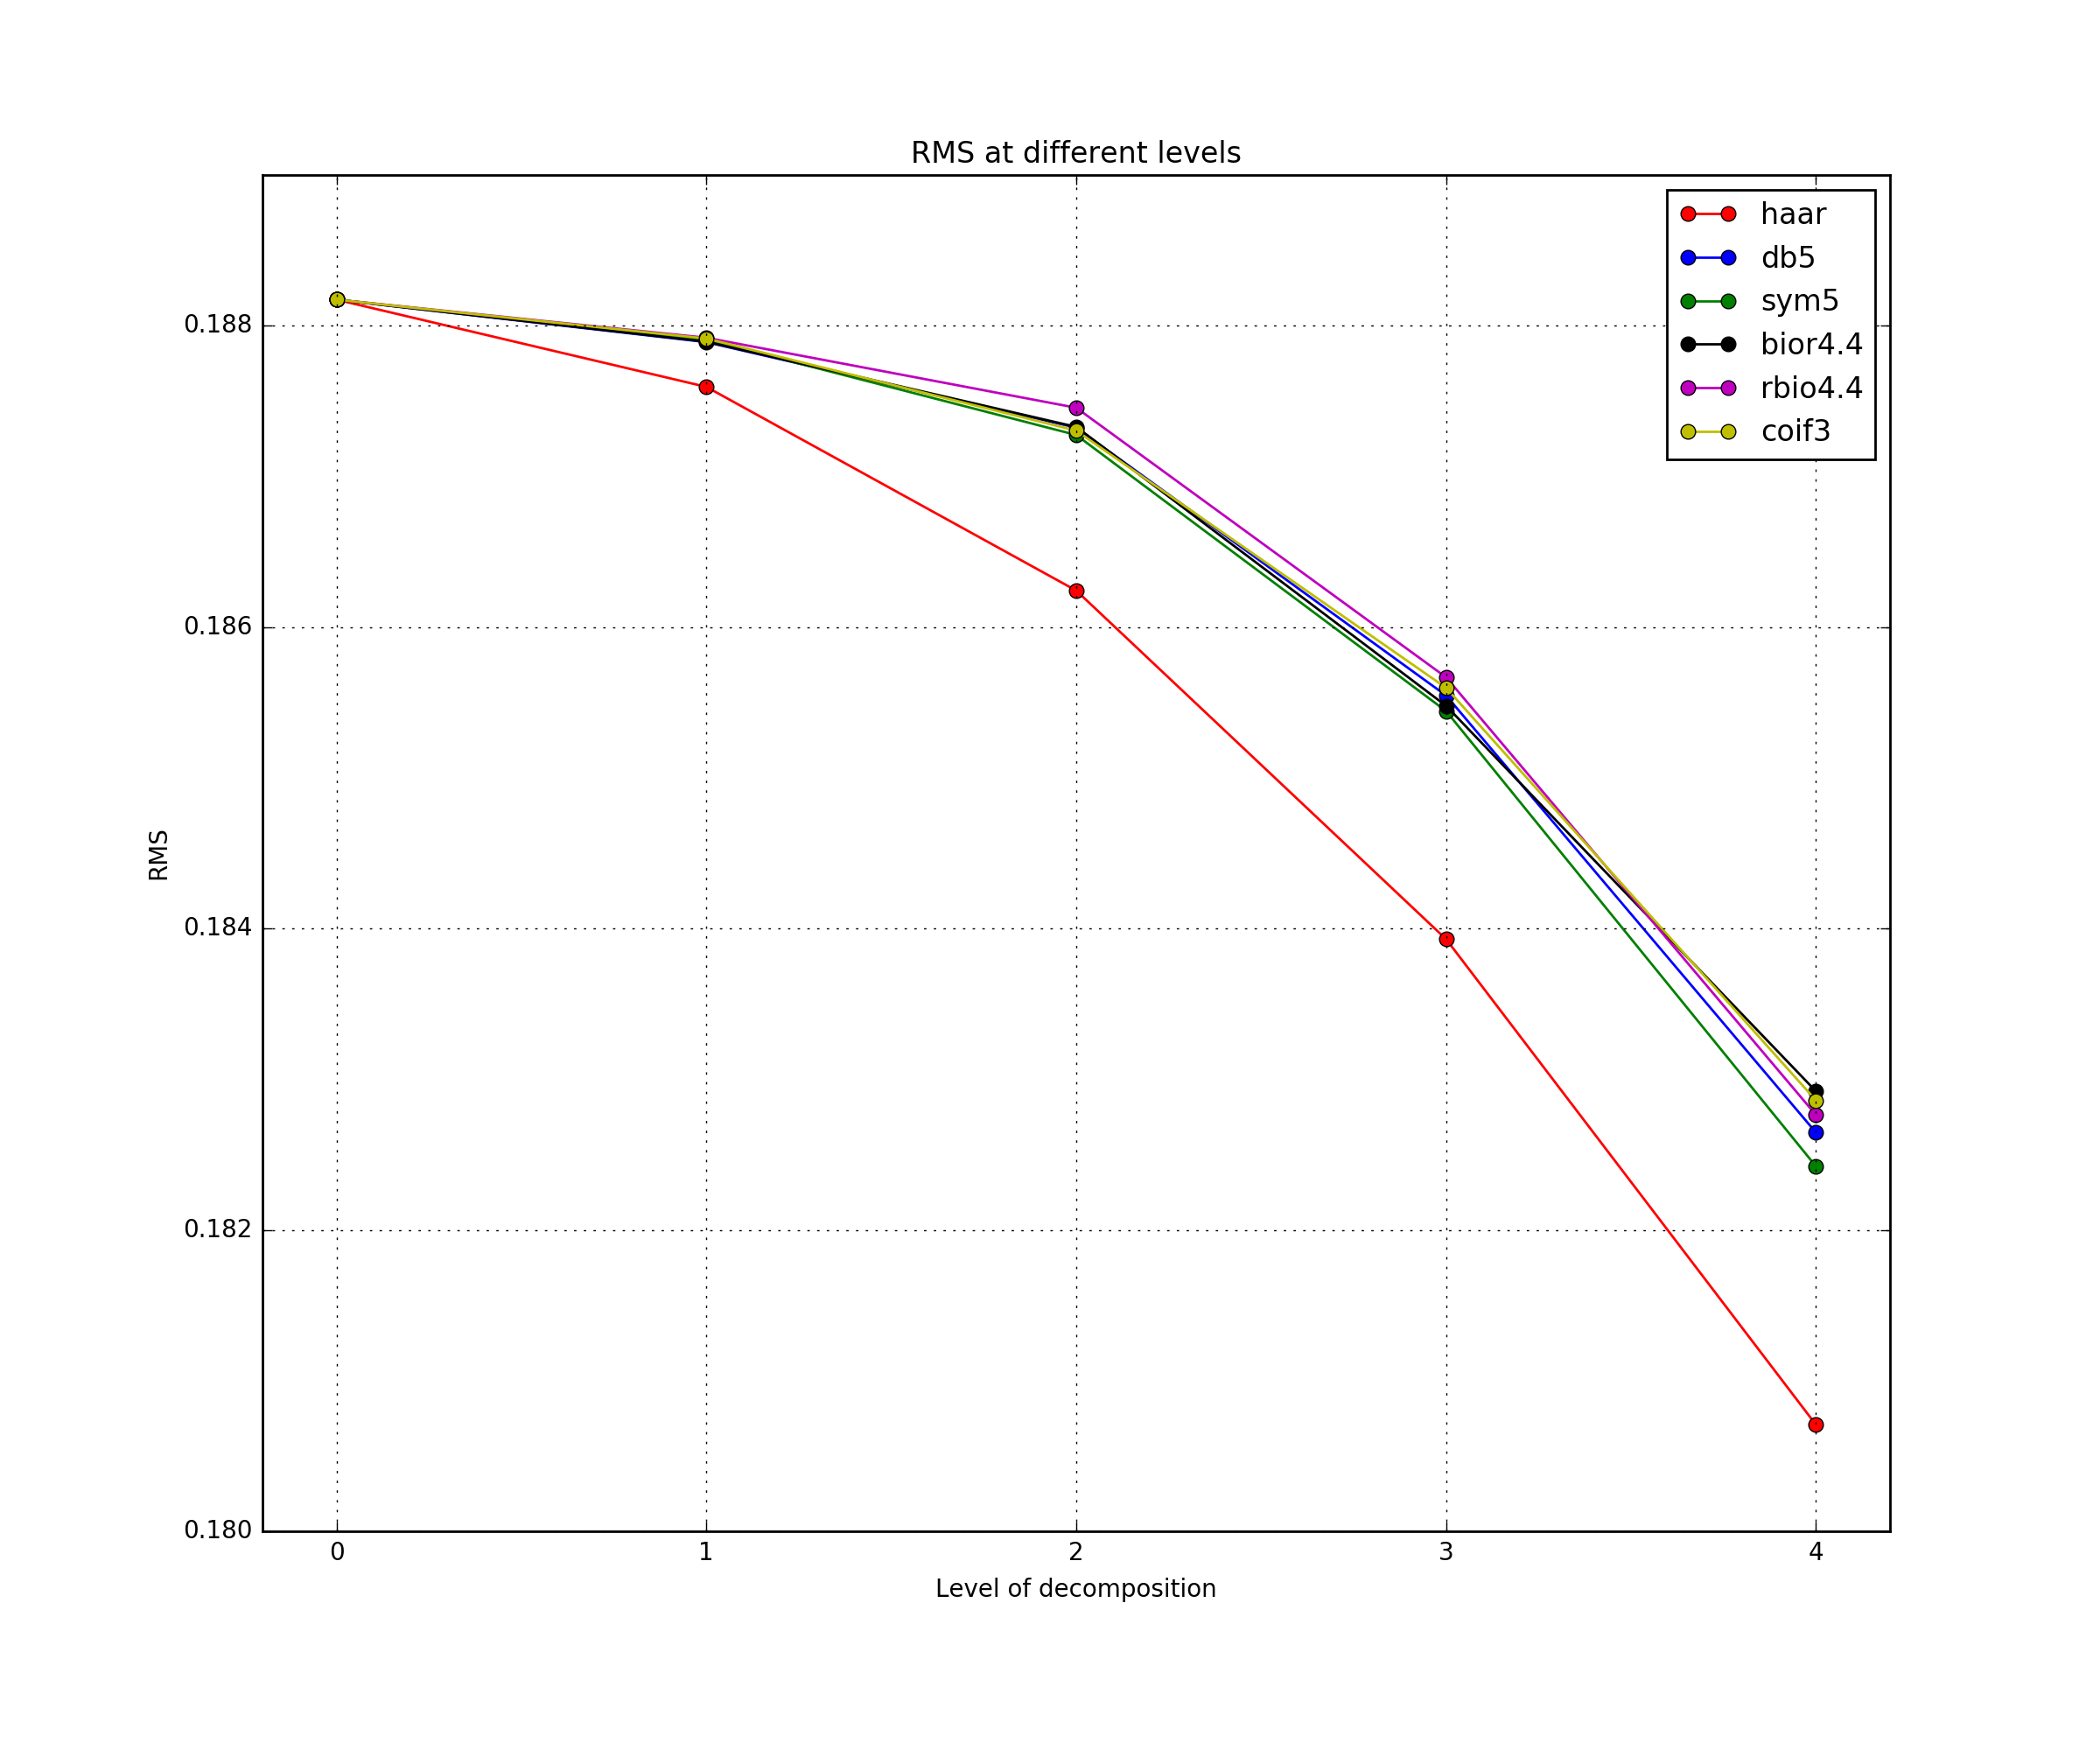
\includegraphics[width=12cm]{rmsgraph}
    \caption{RMS of data decomposed at different levels}
    \label{fig:rms}
    \end{figure}

    A more robust conclusion of the previous phenomenon it is achieved with an analysis of the entropy and the variance of the data and its approximations, as shown in figures \ref{fig:entropy} and \ref{fig:variance} respectively. The entropy (\textit{Shannon entropy}) is a measure of the mean quantity of information contained in the signal, and since the high-pass approximation coefficients stores the fine-grained details of the data, we are dropping out important information and then the entropy is a decreasing function of the decomposition level. Similarly, the fine-grained details are the ones who introduce variability in the data, so it is logical that the variance (measure of the mean variability) decreases by increasing the level of decomposition.
    \begin{figure}[htpb!]
    \centering
    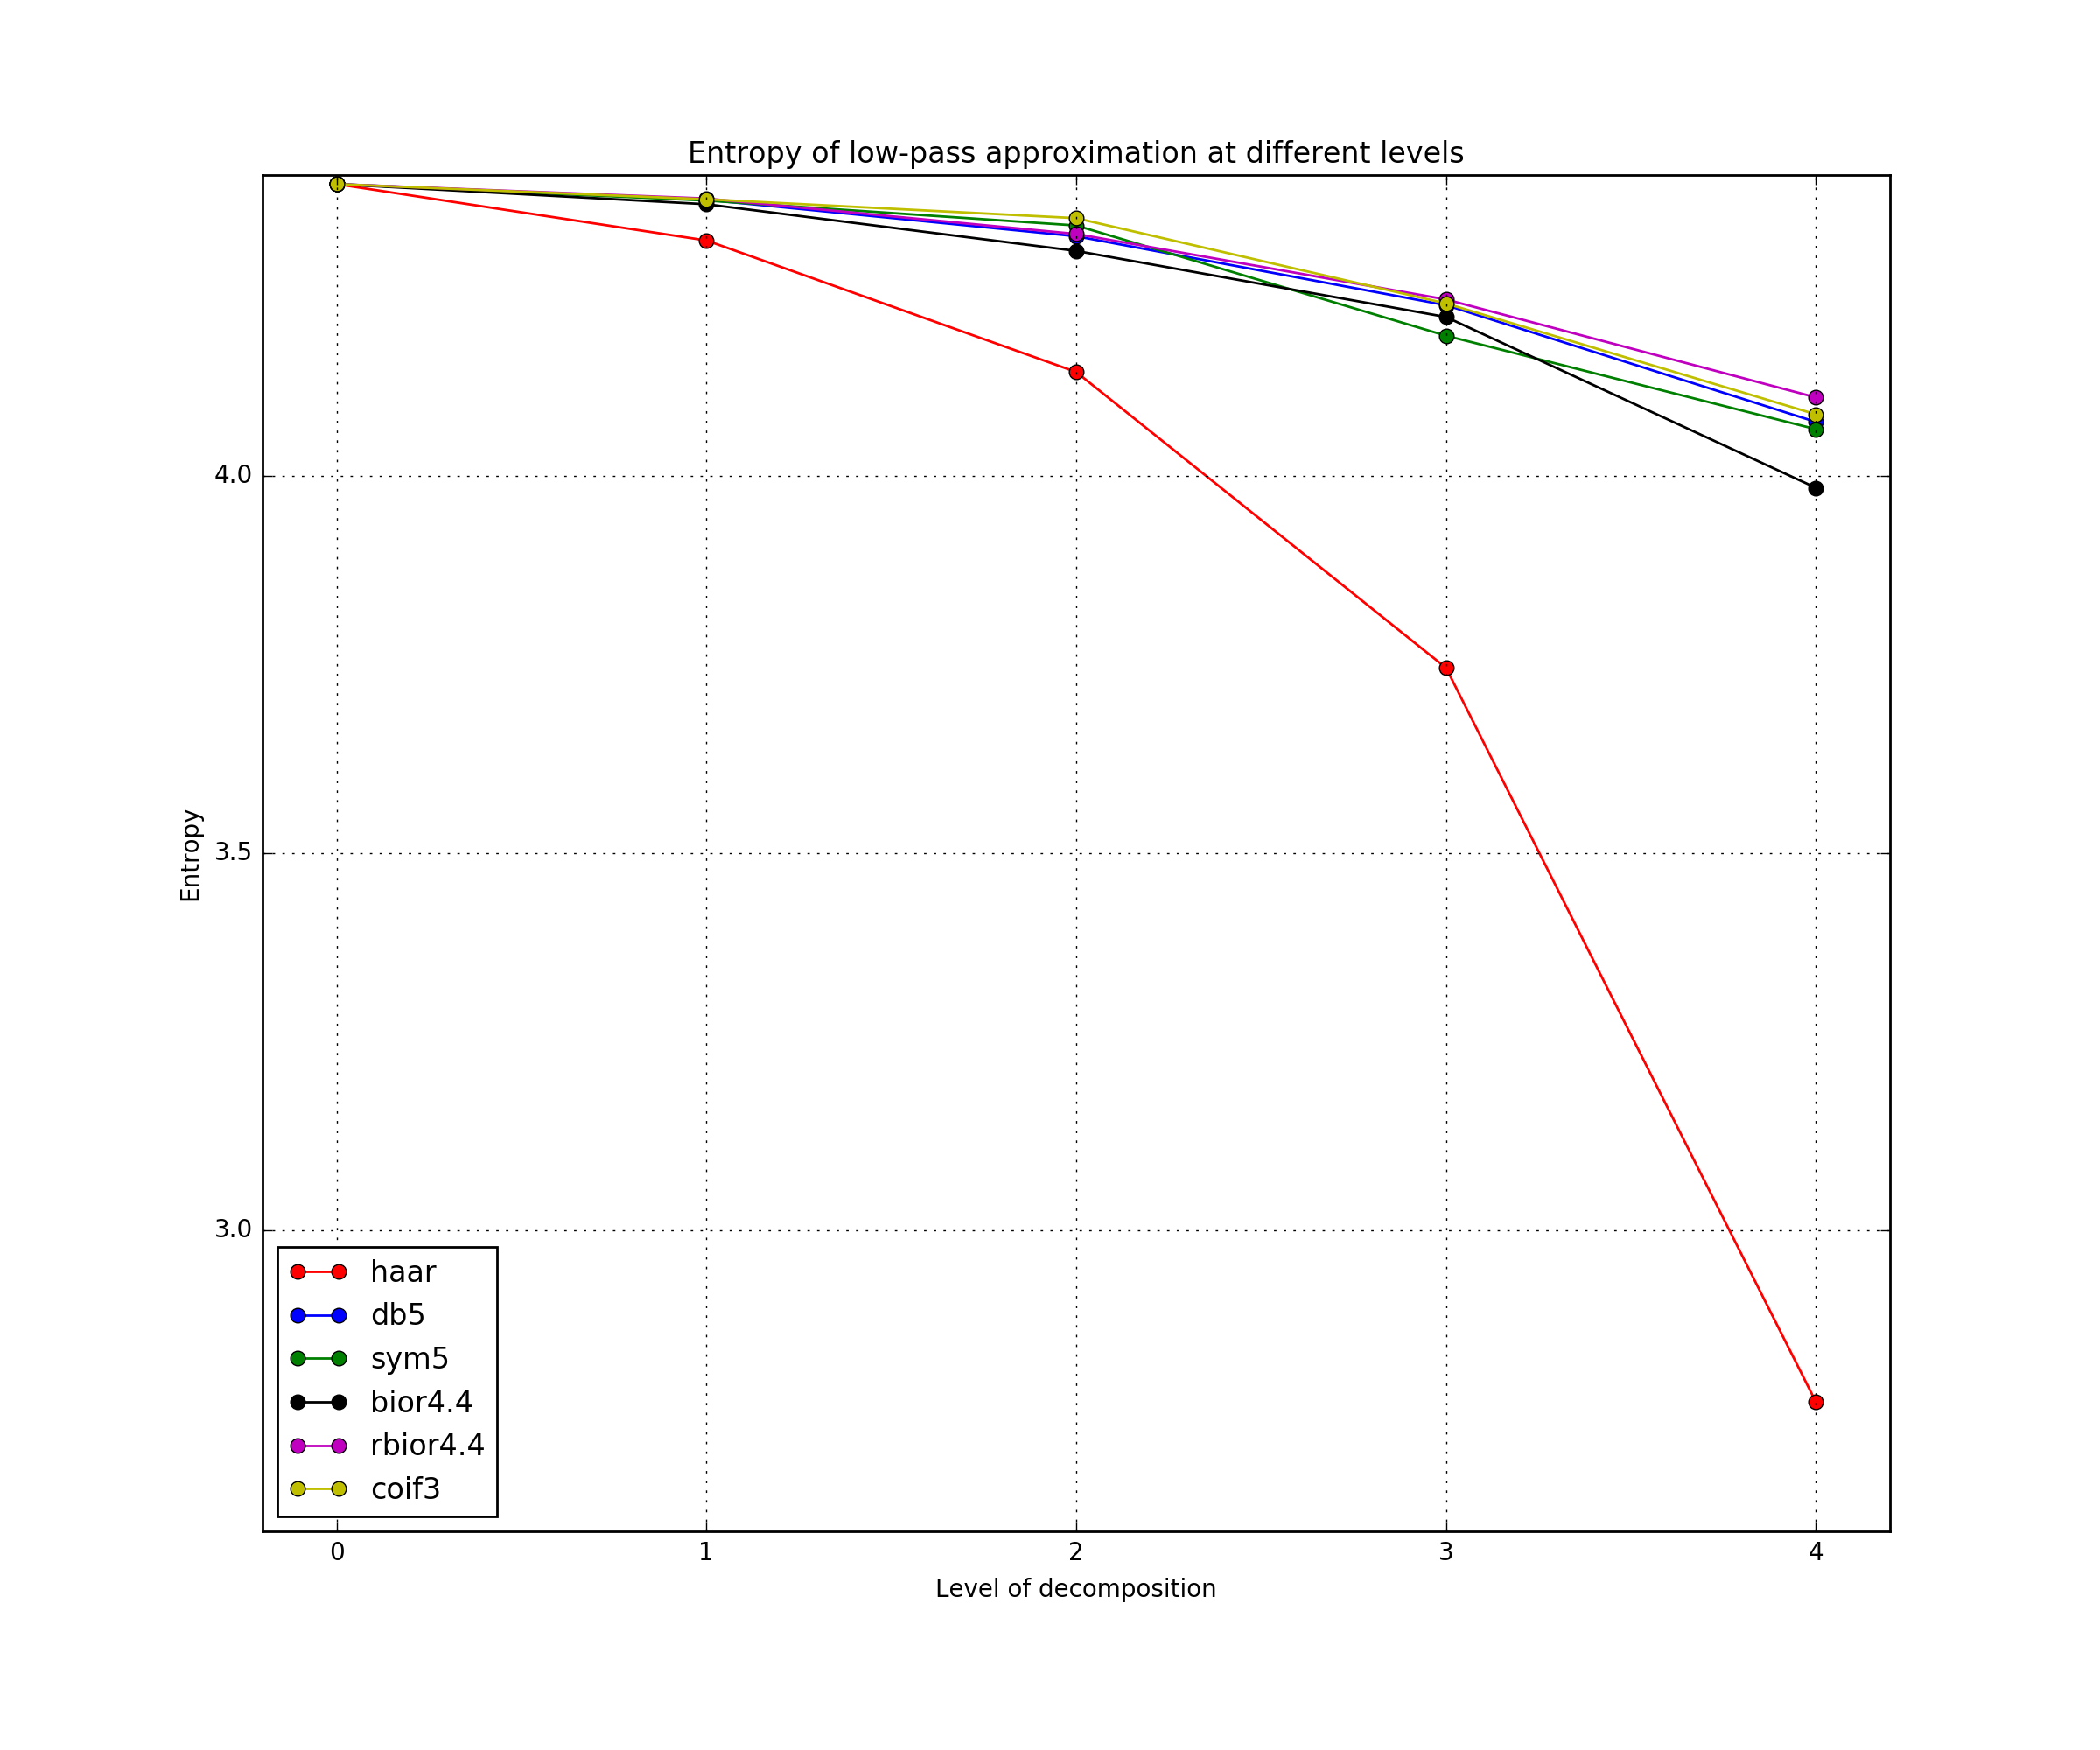
\includegraphics[width=12cm]{entropygraph}
    \caption{Entropy of data decomposed at different levels}
    \label{fig:entropy}
    \end{figure}
    \begin{figure}[htpb!]
    \centering
    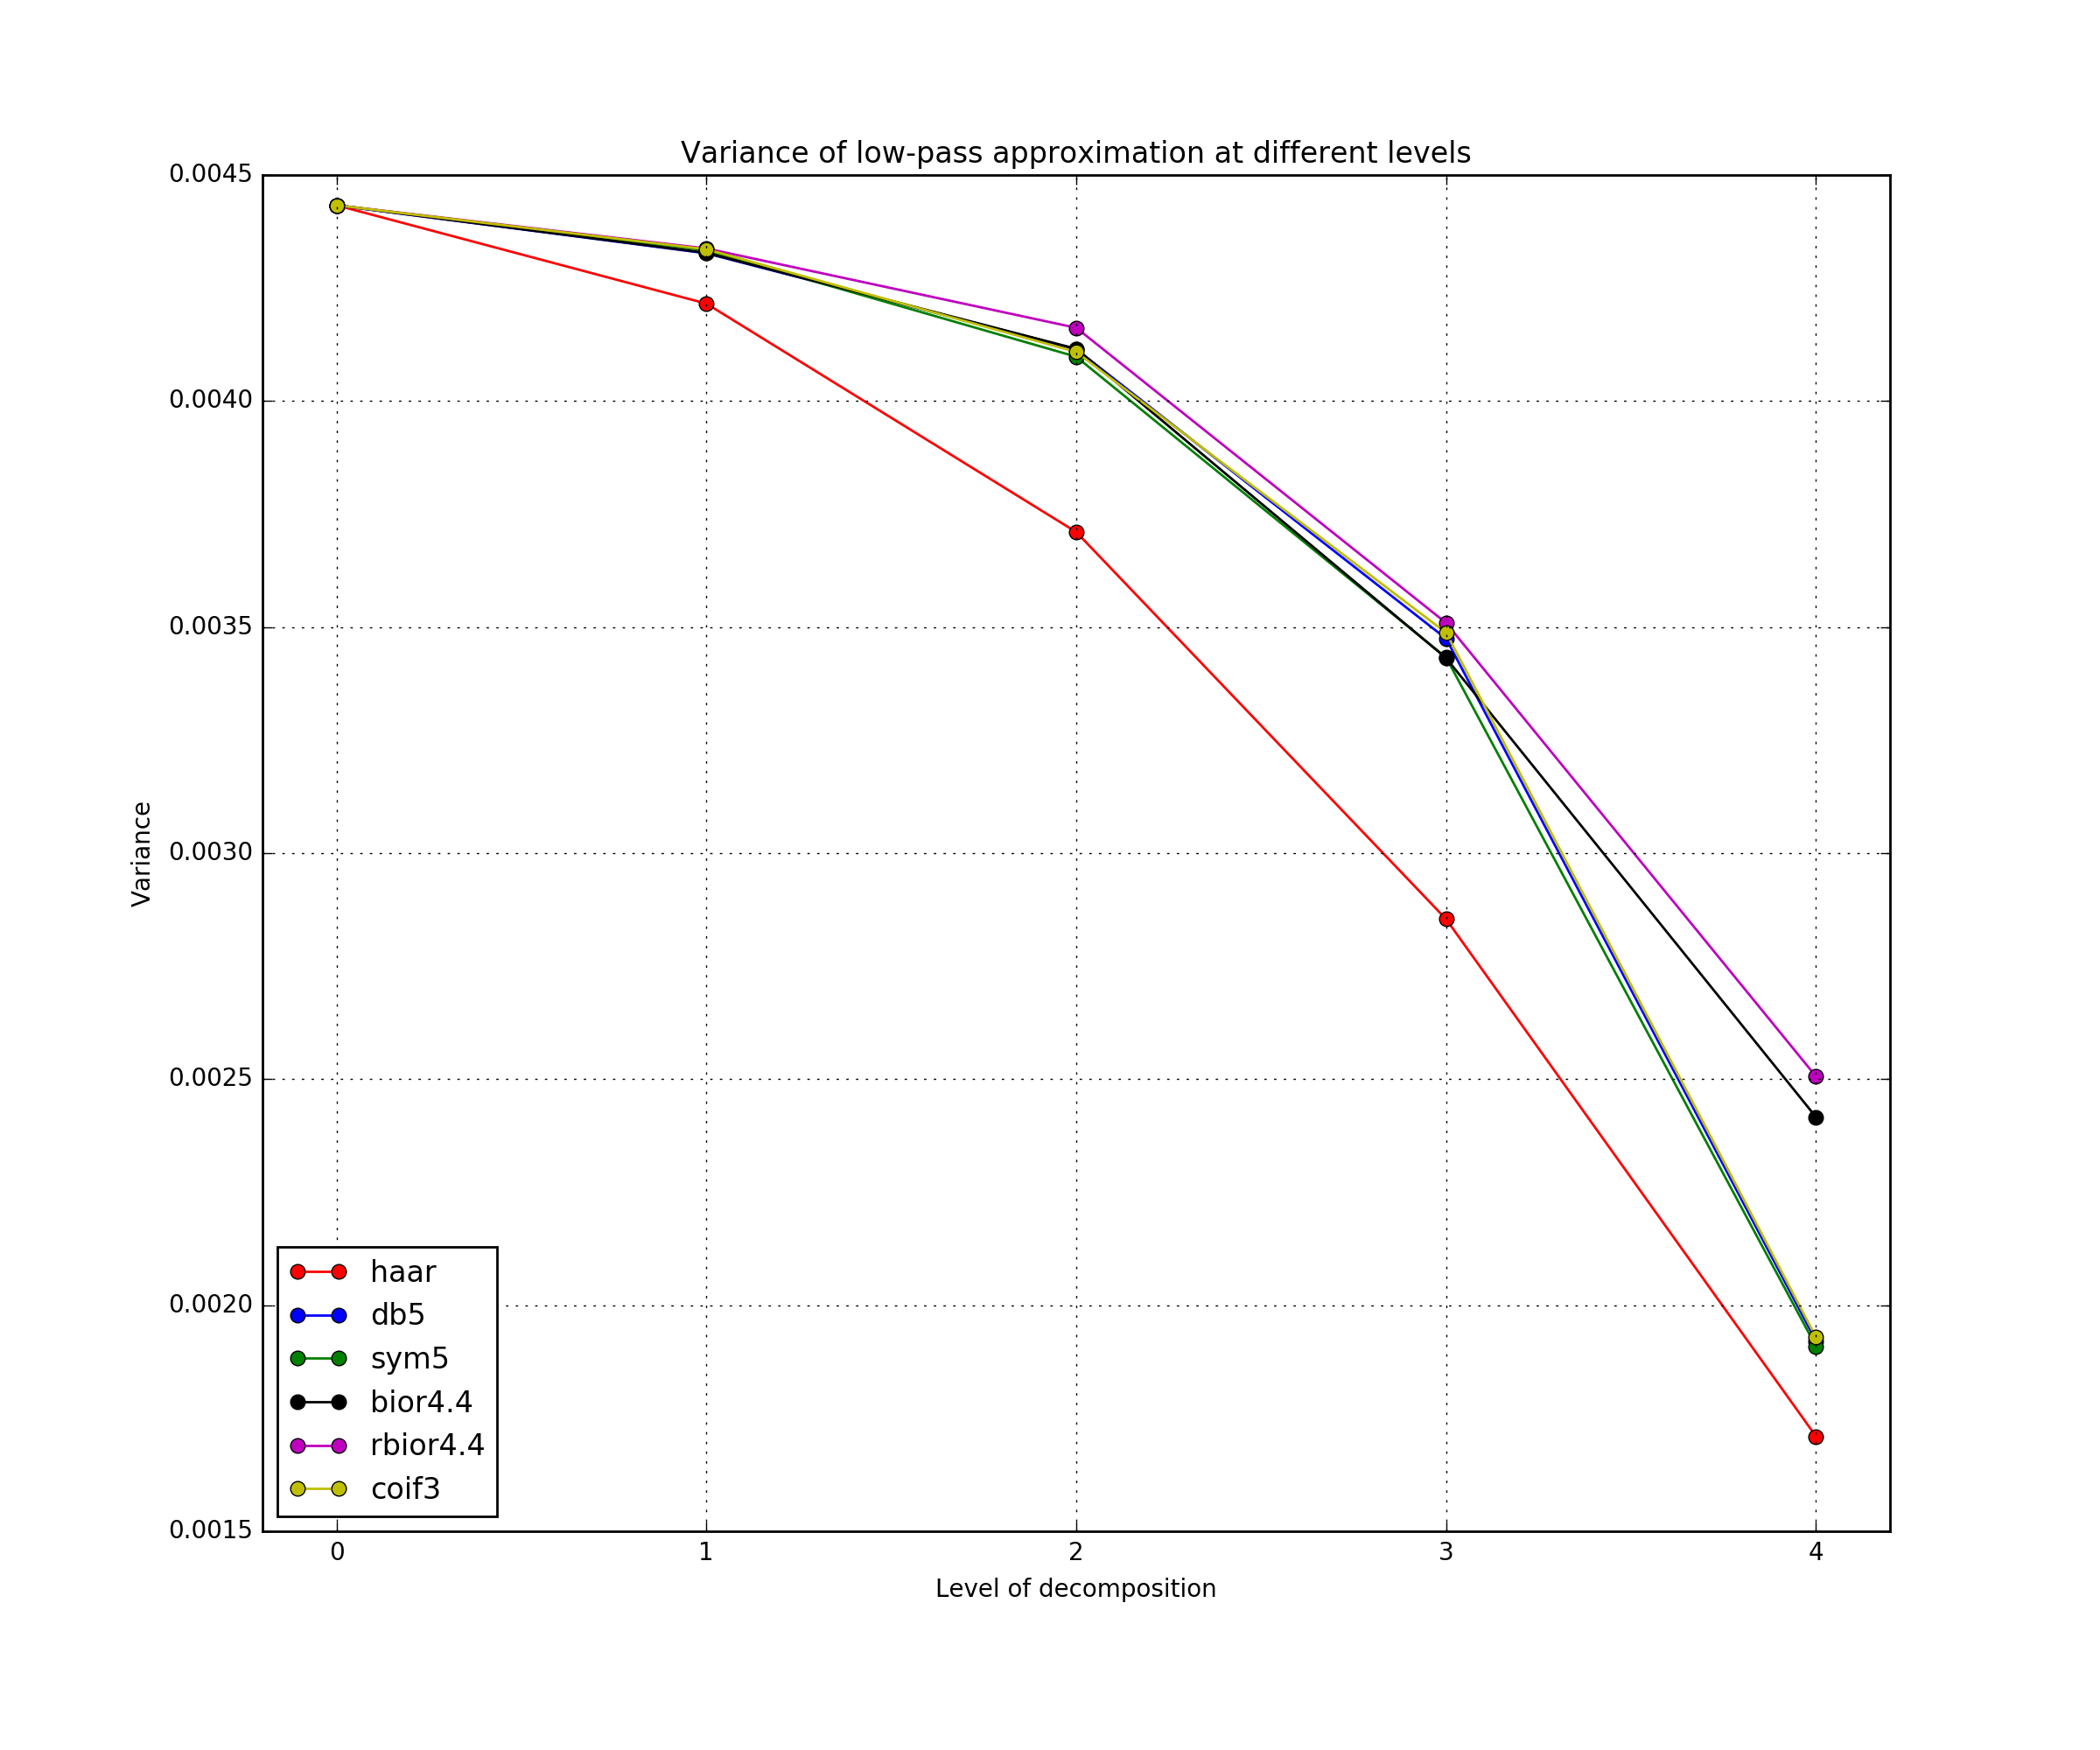
\includegraphics[width=12cm]{variancegraph}
    \caption{Variance of data decomposed at different levels}
    \label{fig:variance}
    \end{figure}

    It is important to note the fast decay of RMS and entropy for the Haar wavelet compared with the rest. This gives a first signal of the drastic behavior of this wavelet, i.e, due to his square shape it loses much information of the signal.



    \item[\textsc{Clumping at Different Levels.}] Because of the RMS variation explained above, two approaches are taken to perform the clumping stage: 1) Compute and use the (decreasing) RMS for each level. 2) Compute the RMS for level $0$ (original data), and use this value for all the levels of decomposition.

    In order to summarize the obtained results, the figures \ref{fig:numclumps}, \ref{fig:maxpix} and \ref{fig:meanpix} shows the number of detected clumps, number of pixels of the bigger clump and  the mean number of pixels of the clumps, respectively.  

    \begin{figure}[htpb!]
    \centering
    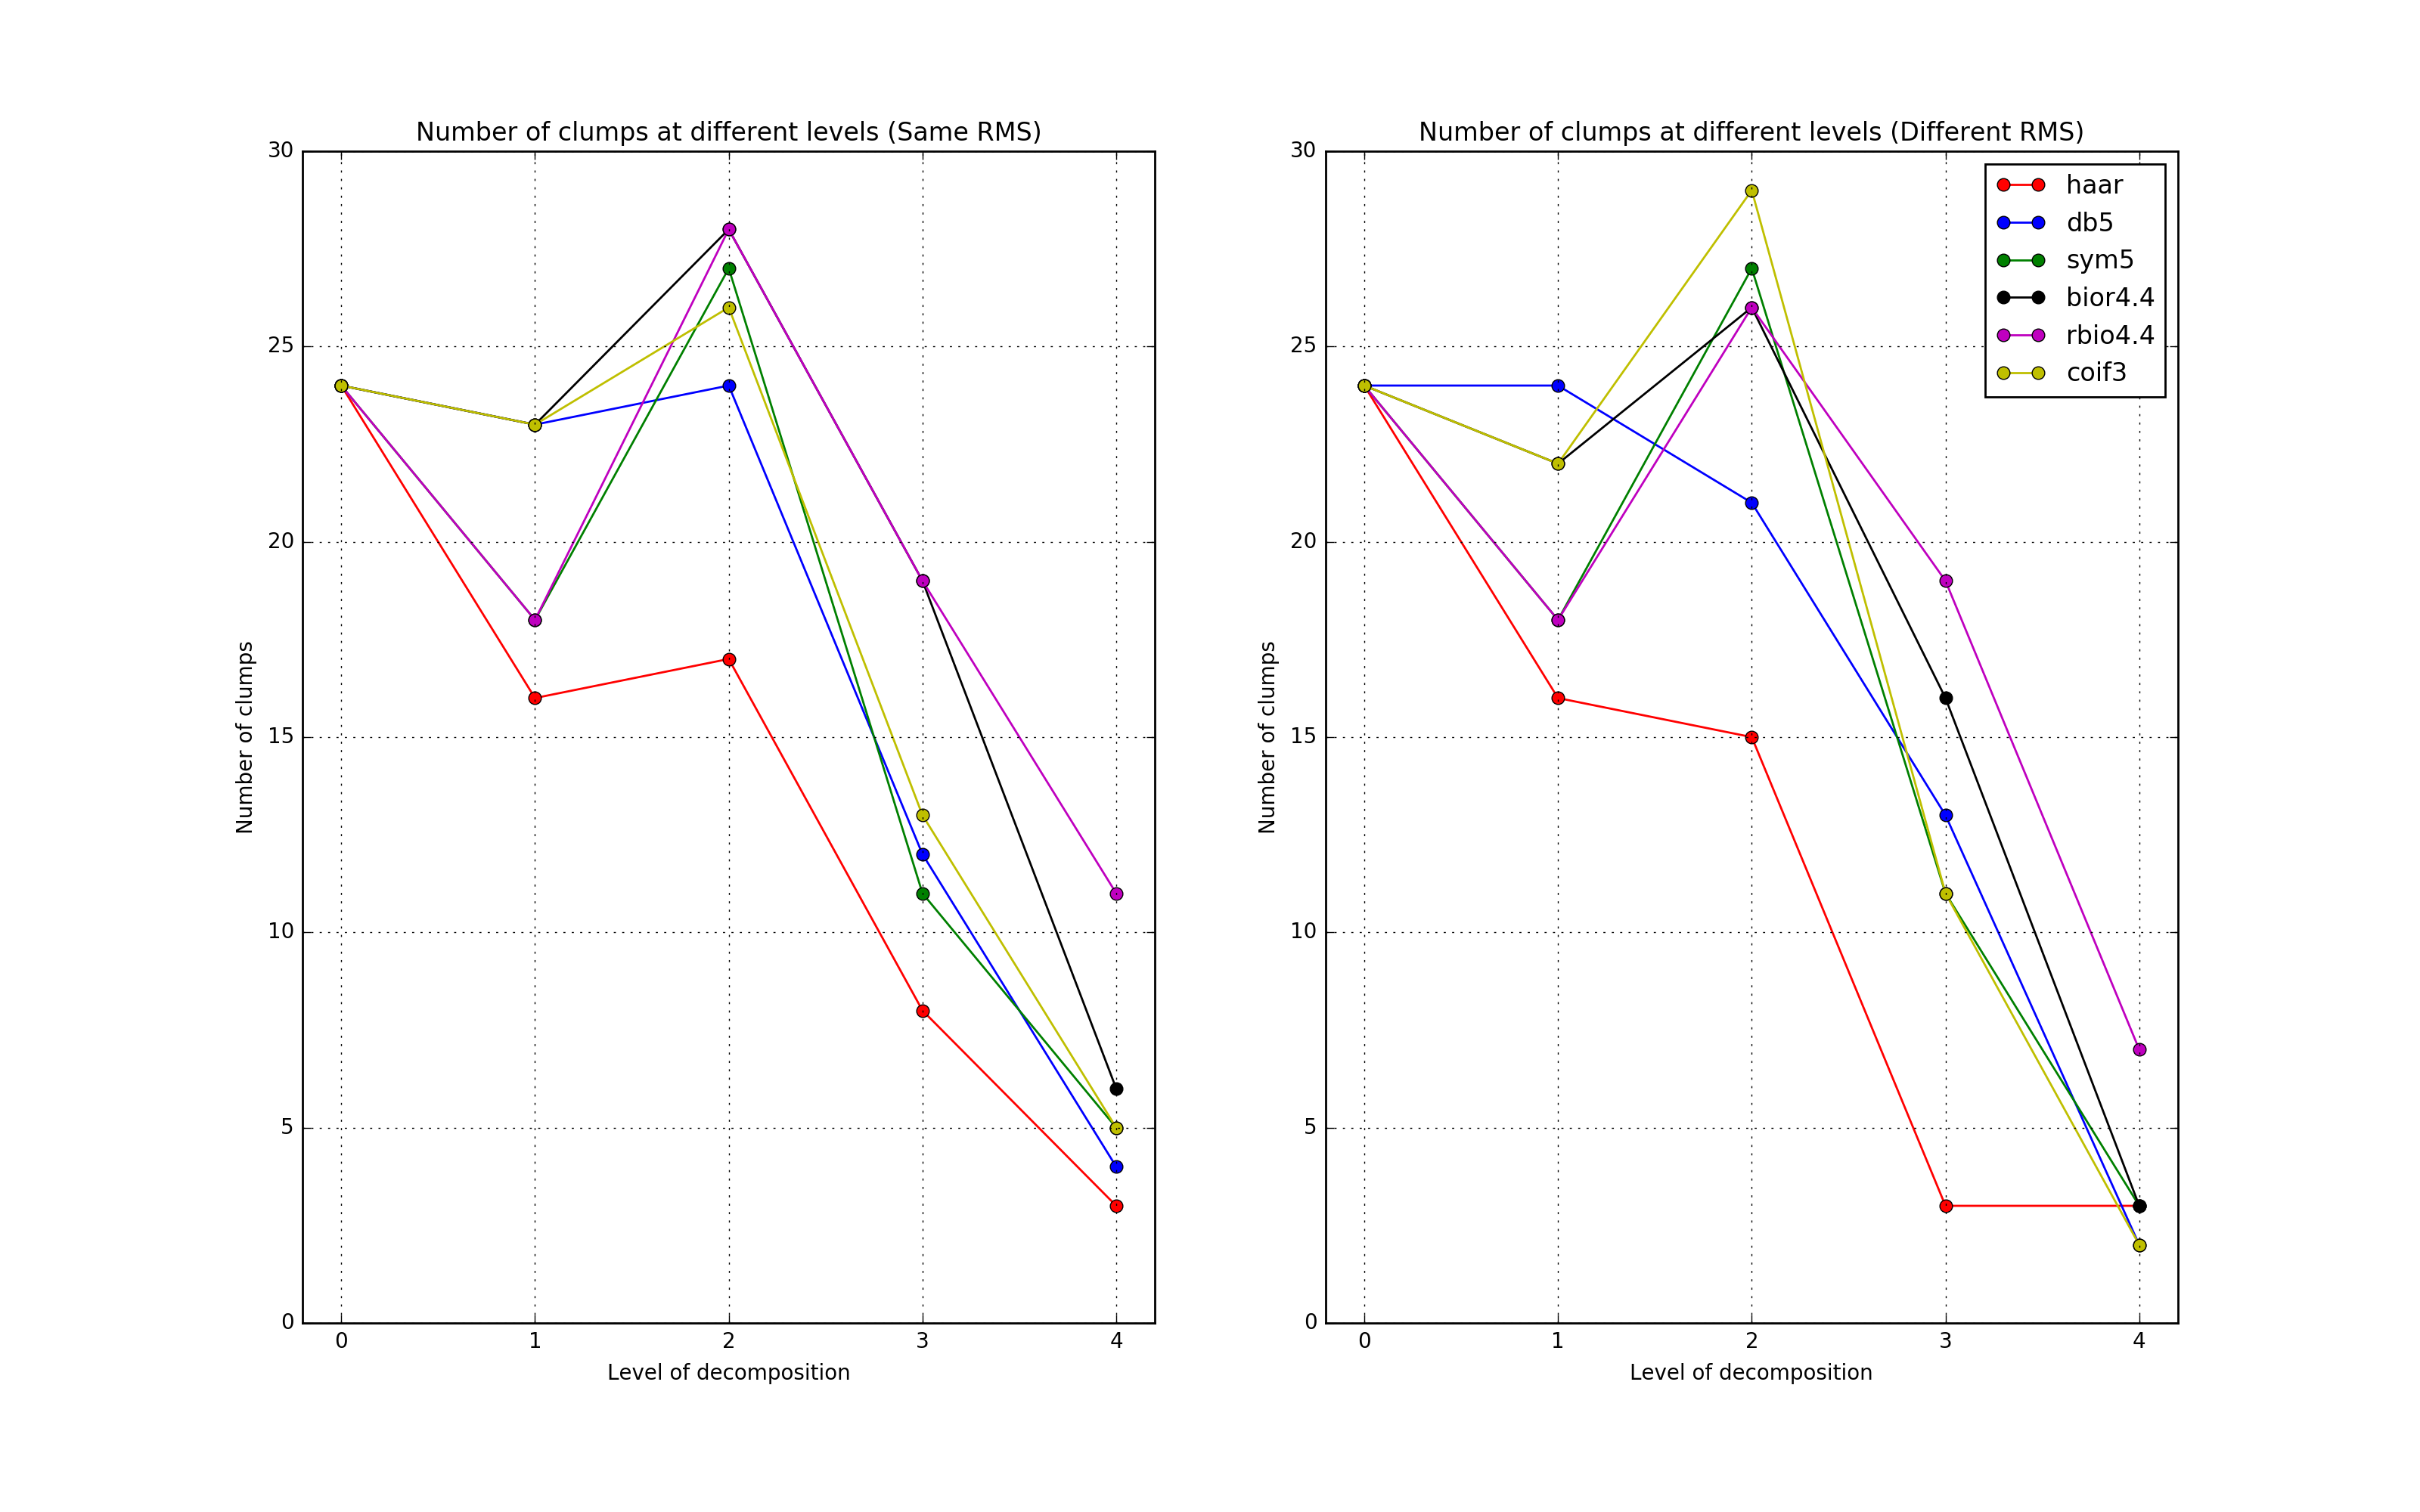
\includegraphics[width=17cm]{numclumpsgraph}
    \caption{Number of detected clumps at different levels}
    \label{fig:numclumps}
    \end{figure}
    \begin{figure}[htpb!]
    \centering
    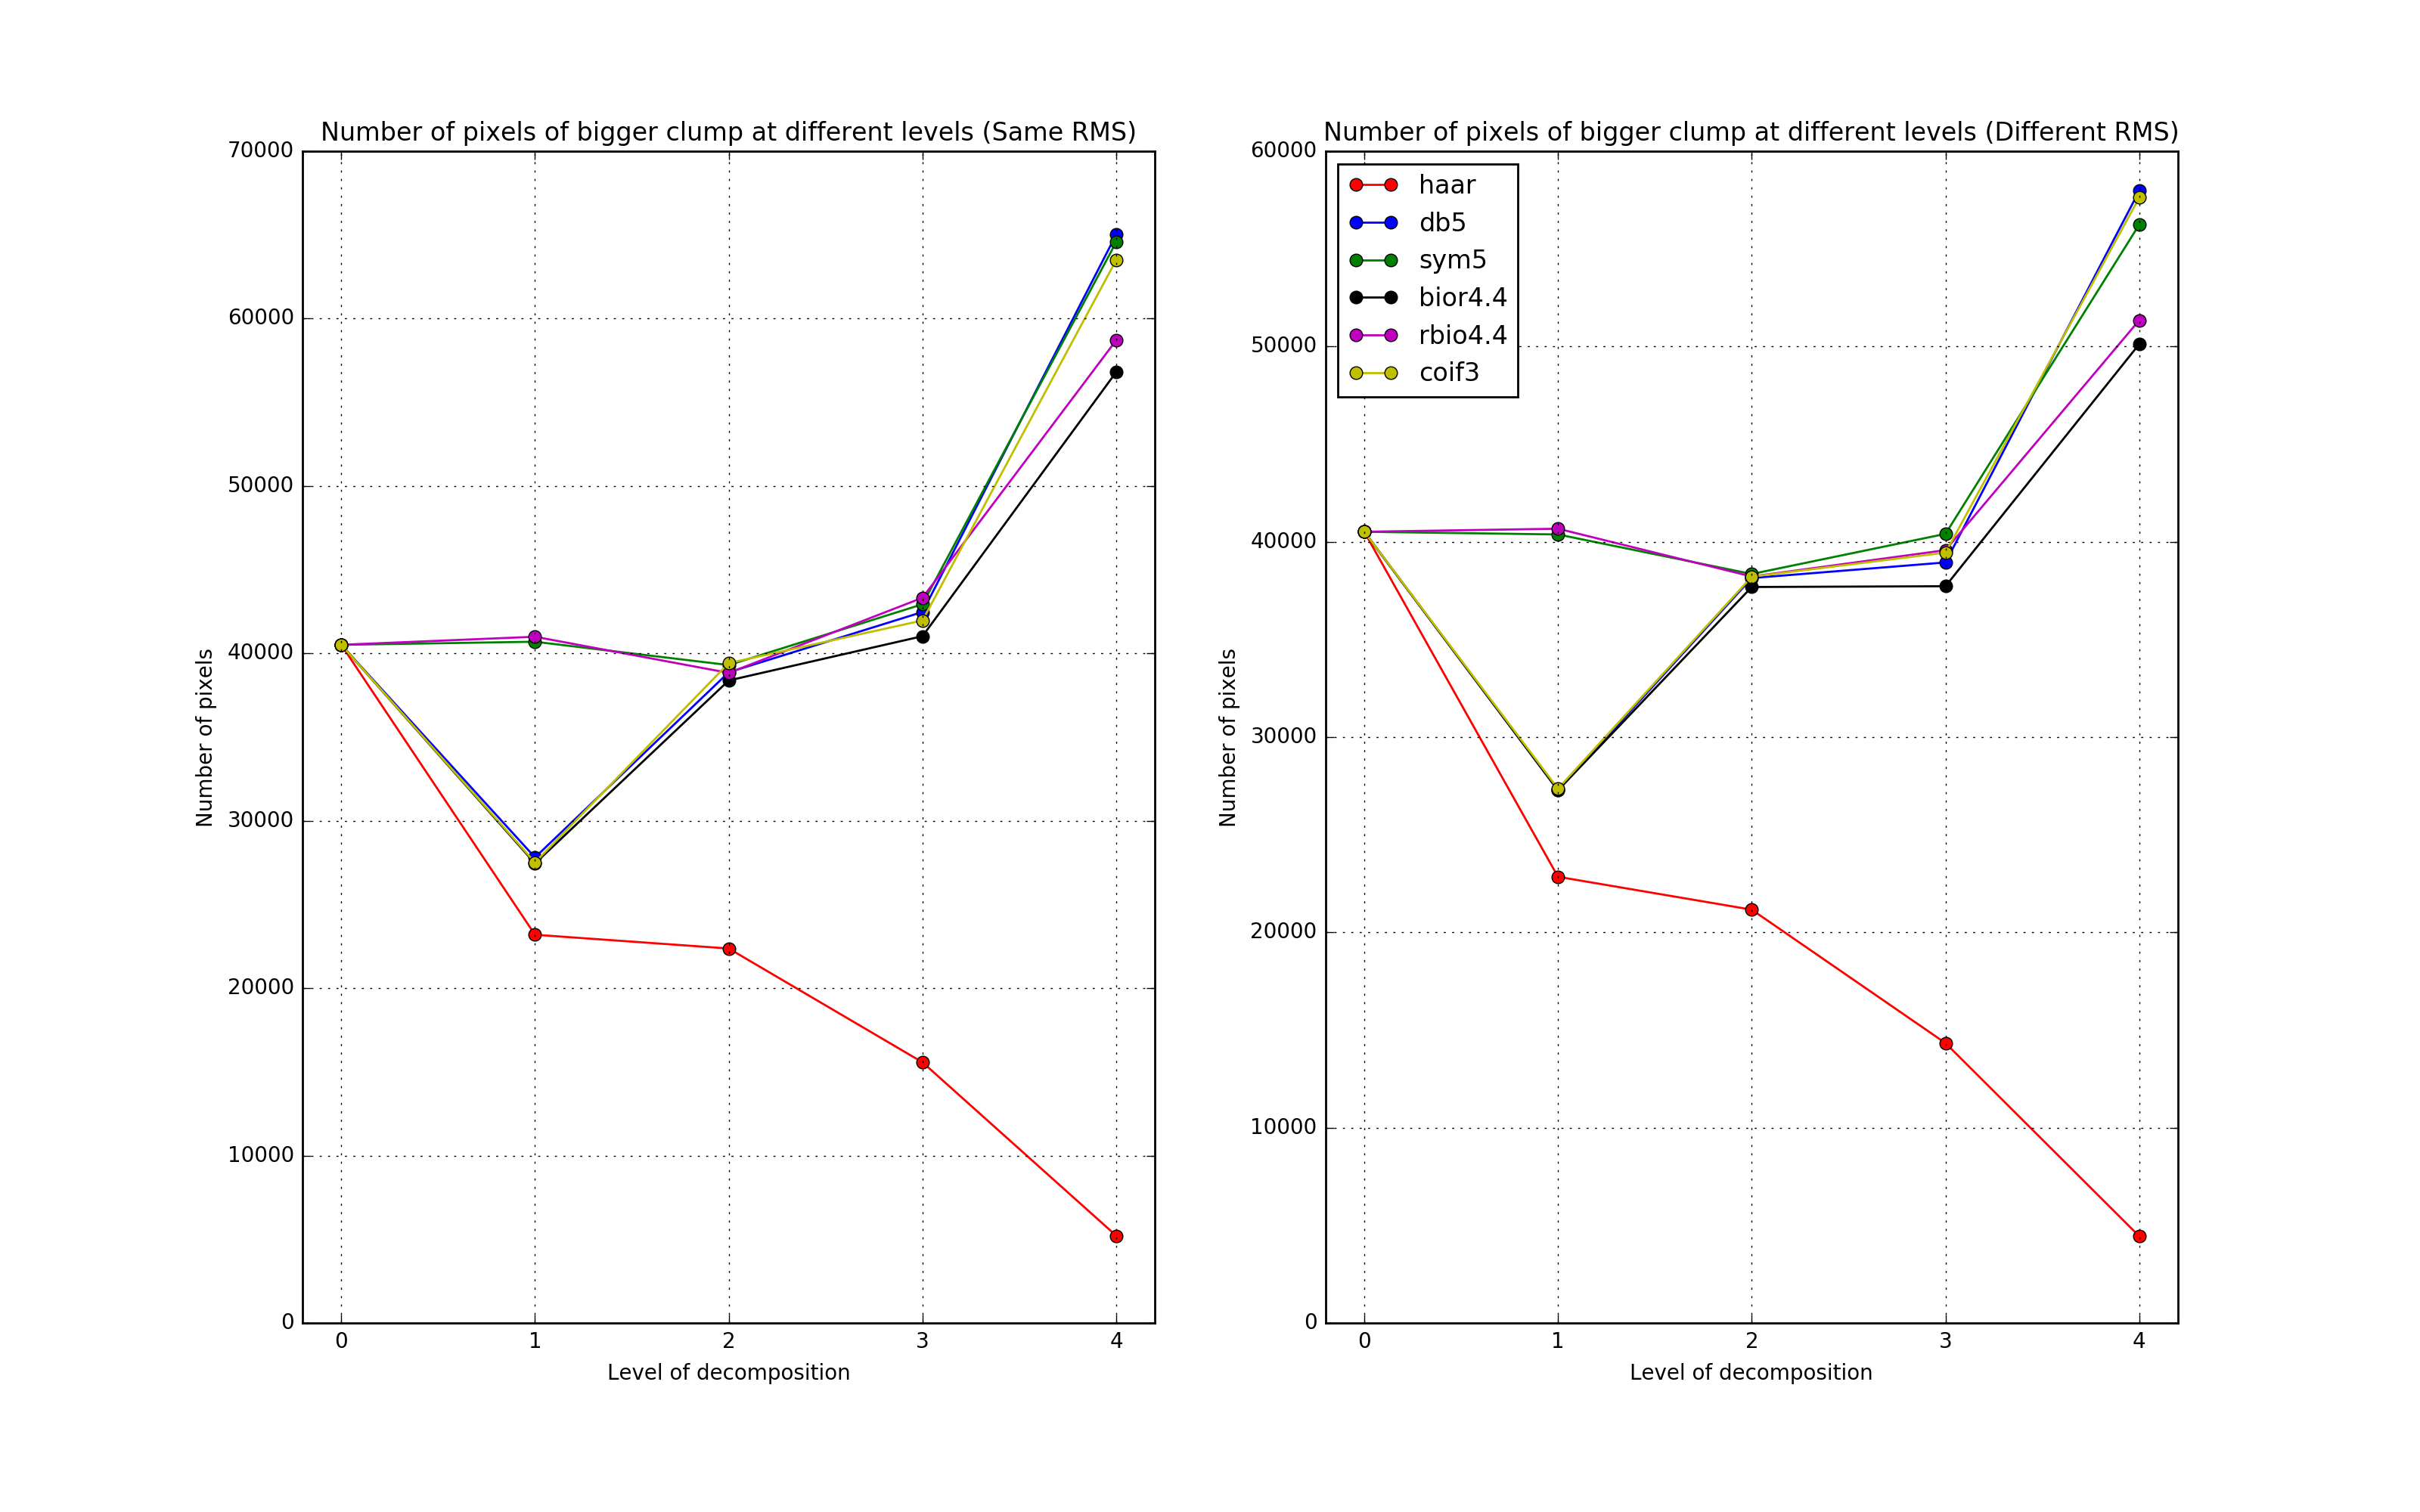
\includegraphics[width=17cm]{numpixgraph}
    \caption{Number of pixels of the bigger detected clump at different levels}
    \label{fig:maxpix}
    \end{figure}
    \begin{figure}[htpb!]
    \centering
    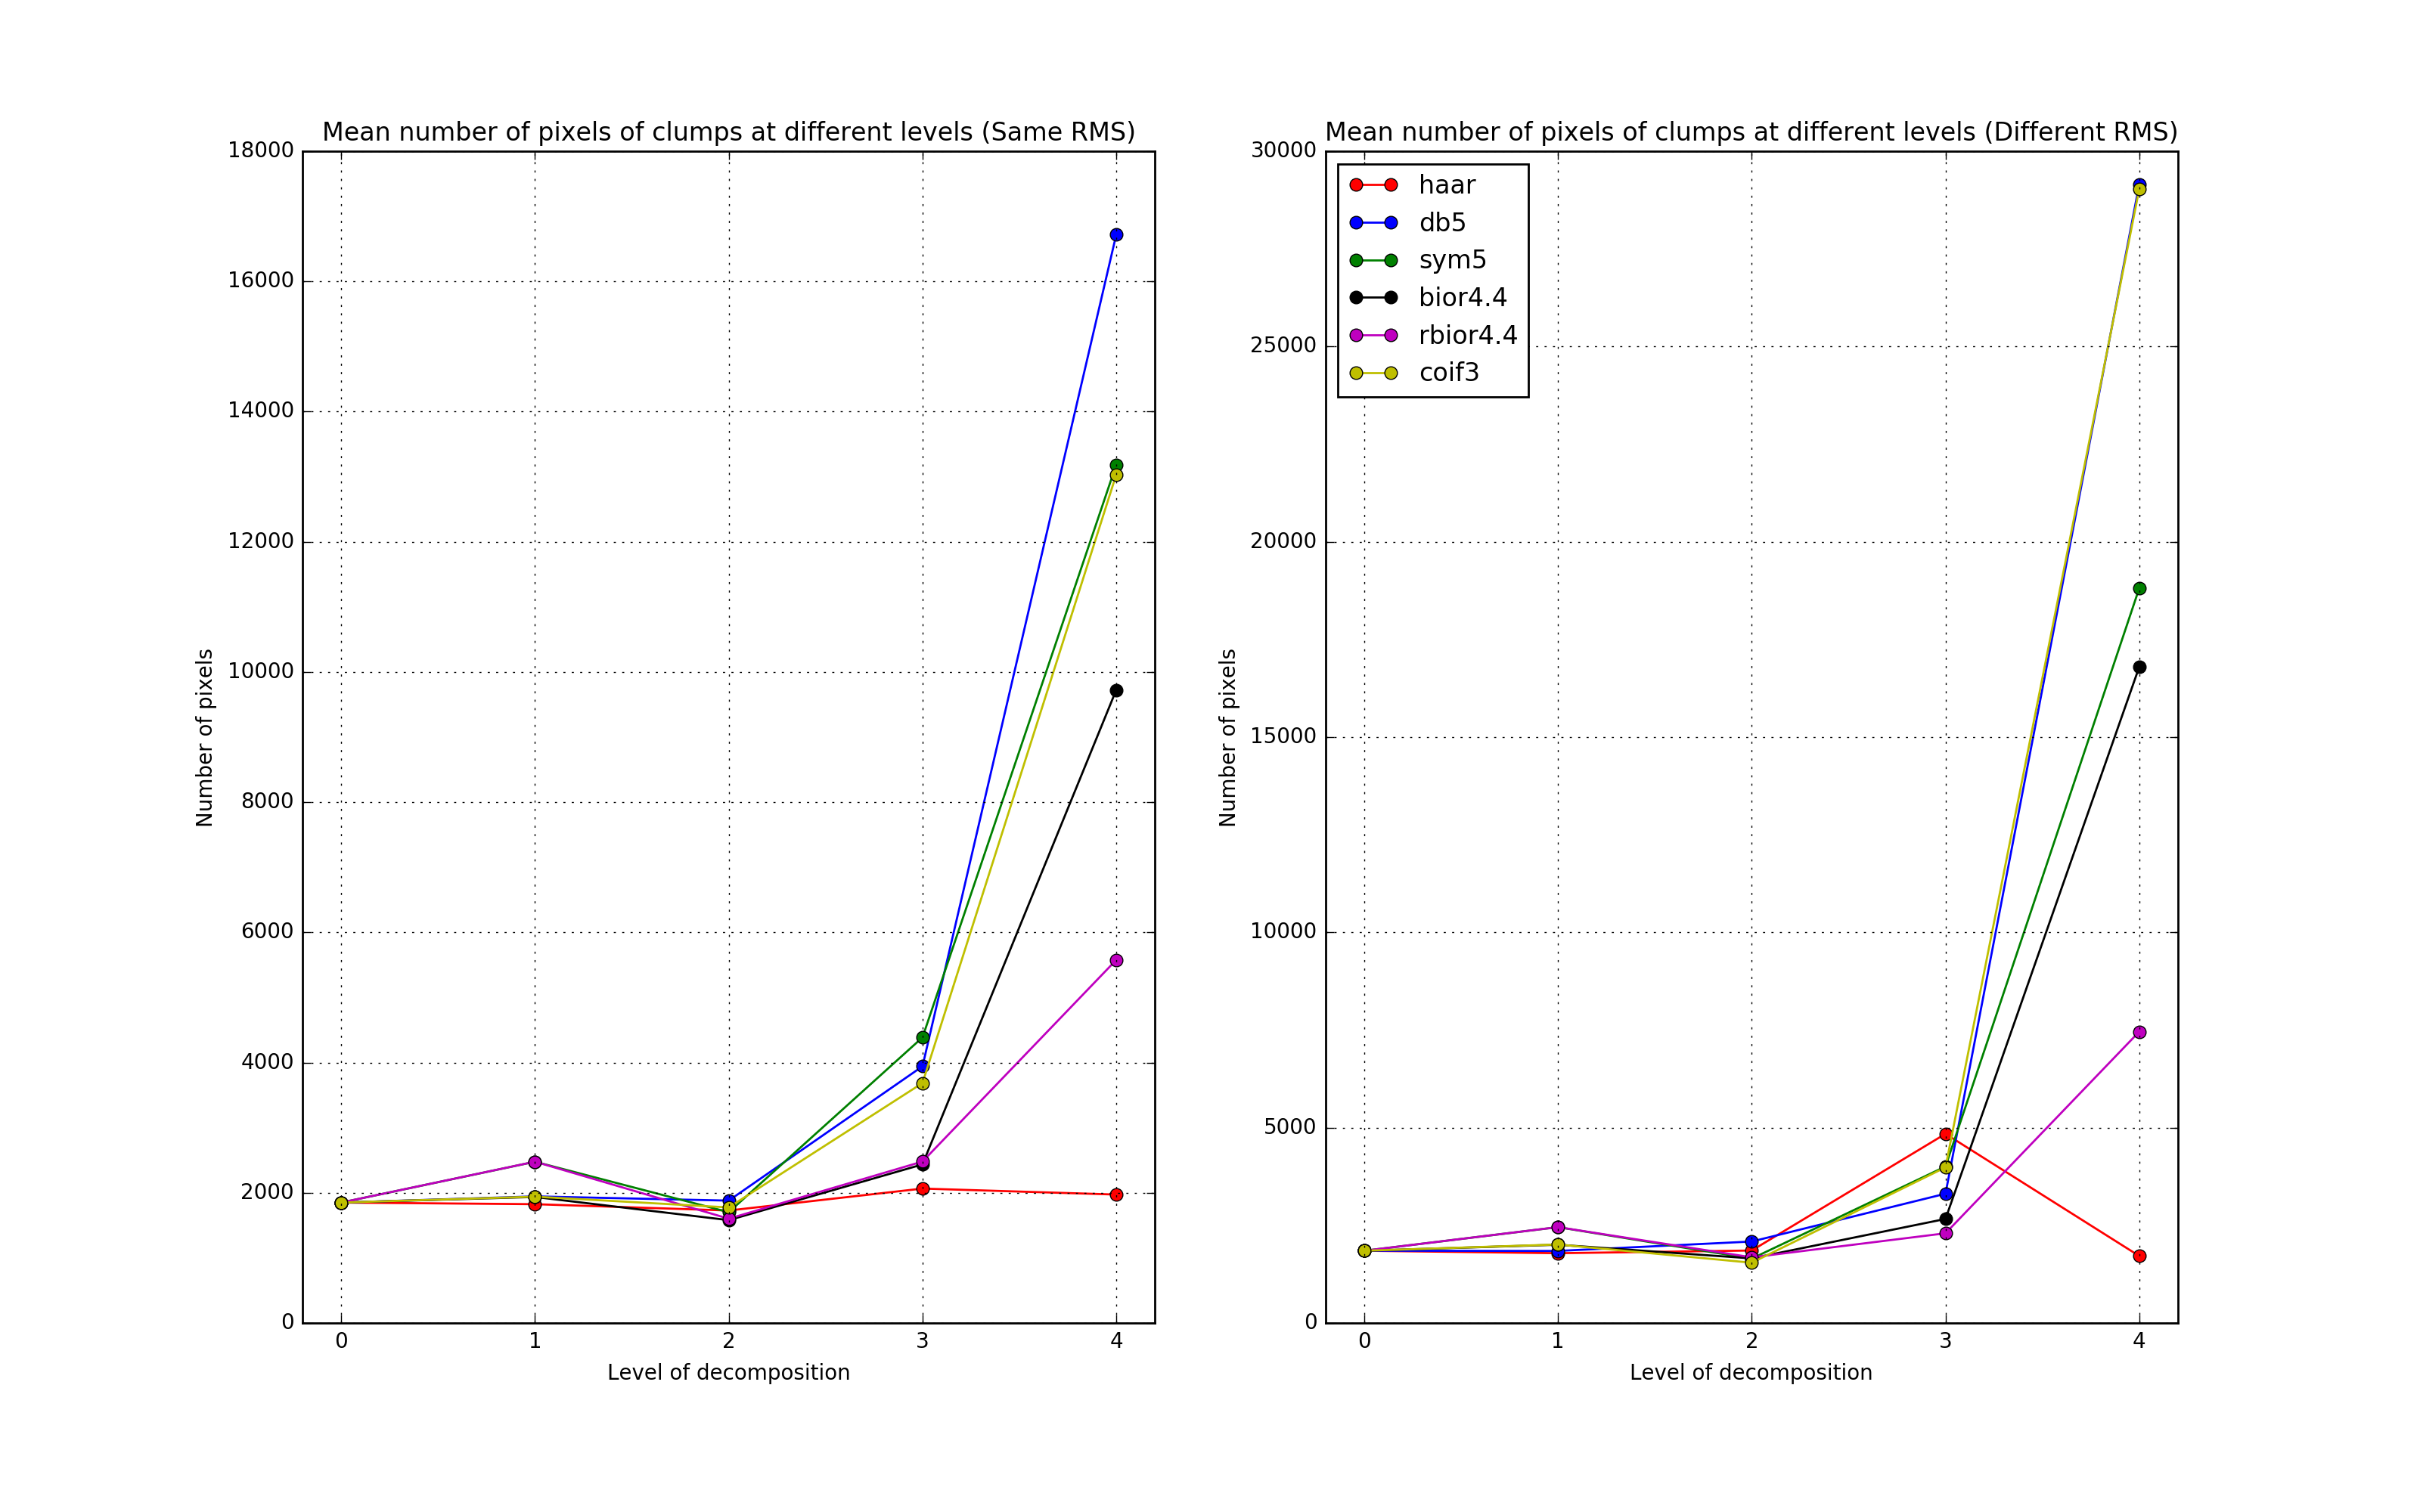
\includegraphics[width=17cm]{meanpixgraph}
    \caption{Mean number of pixels of clumps detected at different levels}
    \label{fig:meanpix}
    \end{figure}

    Based on the results, we can state the following:
    \begin{itemize}
        \item There is a decreasing tendency for the number of detected clumps, which is the expected behavior. However, at intermediate levels (level $2$), there is an increase for almost all wavelets.
        \item There is an increasing tendency for the number of pixels of the bigger clump, and the mean number of pixels per clump, which (again) is the expected behavior. The only exception is the Haar wavelet, that shows an opposite behavior. This supports our first conclusion about the Haar wavelet: Is not doing a good job representing the data.
        \item Noticeable differences are observed between the two approaches for the RMS value. In particular Figure \ref{fig:meanpix} shows a huge change between the mean number of pixels per clump, that supports our hypothesis about the changing behavior of the clumping algorithms with the RMS. The main reason for the difference, is due to the thresholding stage of Fellwalker, where all the pixels above some multiple of the RMS are set as unusable. Since the second approach (variating RMS) has decreasing RMS value, it takes more pixels as usable, and therefore the mean number of pixels per clumps increases too.  
    \end{itemize}



    \item[\textsc{Hierarchical relations.}] For the representation of the hierarchical relations between the clumps detected at different levels, a tree structure is used as shown in Figure \ref{fig:htree} \footnotemark[1]. The clumps at the top of the three corresponds to structures detected on data at the higher level of MRA, i.e, with coarse-grained details, and the clumps at the bottom of the three, are the ones detected in the original data. 

    \begin{figure}[htpb!]
    \centering
    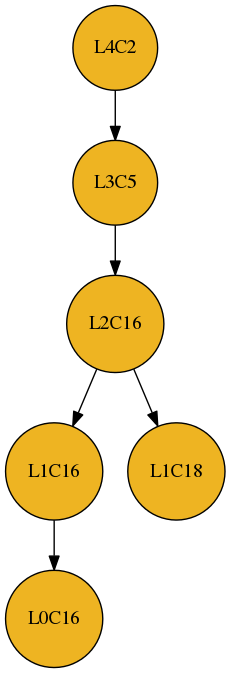
\includegraphics[width=3cm]{sub_htree}
    \caption{Portion of the hierarchical tree structure}
    \label{fig:htree}
    \end{figure}

    The labels of the nodes have the following structure: $\text{L}\{\texttt{level number}\}\text{C}\{\texttt{clump identifier}\}$, indicating the level of decomposition and the identifier of the detected clump at this level.

    From the tree structure above it is possible to visualize graphically the relation between the clumps, as shown in Figure \ref{fig:3Dplot}. Here we plot L2C16 (cyan), L1C16 (green) and L1C18 (brown). As expected, the L2C16 clump encloses the other two, i.e, when we perform clumping with more detailed data, the original clump is splited into two separated structures.   

    \begin{figure}[htpb!]
    \centering
    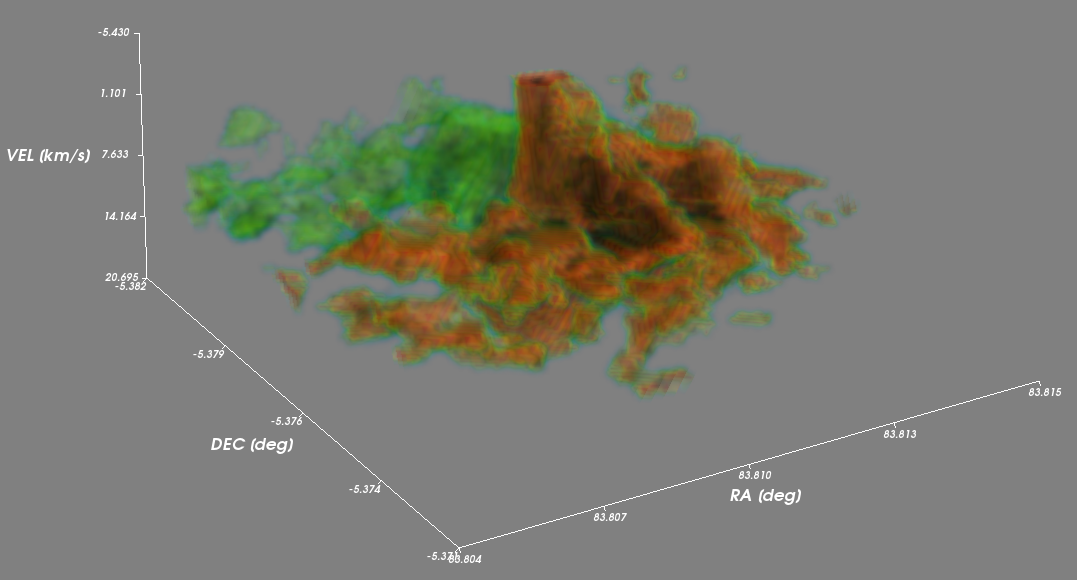
\includegraphics[width=12cm]{3Dplot}
    \caption{3D visualization of L2C16, L1C16 and L1C18}
    \label{fig:3Dplot}
    \end{figure}


    \footnotetext[1]{This is just a part of the whole tree. The complete hierarchical tree can be seen \href{https://github.com/mavillan/WavClump/tree/master/src/htree.png}{here}}

\end{description}


\newpage
\section{\textsc{Conclusions and future work}} \label{conclusion}

In this work, we have implemented and studied a multiresolution analysis with different Wavelet families, over standard astronomical data, with the aim of performing clumping algorithms with this data at different levels of details, so we can determine the hierarchical relation between the structures detected between levels.


The main contribution was the implementation of the multiresolution analysis over 3D data cubes by using the 3D DWT, since the SWT becomes an unfeasible alternative for 3D data, due to the redundancy of the approximation coefficients.

As explained in Section \ref{experiments}, the process of image reconstruction through the approximation coefficients successively obtained, allows us to generate coarse-grained versions of the original data, since at each step high frequency characteristics are being dropped out.

One of the main faced problems, was the dependency of the clumping algorithm (Fellwalker) with the RMS, and the inverse relation of the RMS with the level of decomposition of the approximated data. By studying the variance and shannon entropy of the reconstructed data, we empirically check a theoretical fact about the MRA process: At each level, more fine-grained (high-frequency) details are dropped out of the signal, and so the RMS, variance and entropy decreases as well. Because of that, we test two clumping approaches: dynamic RMS (computing it at each level) and static RMS (keeping the same as level $0$). These two approaches showed significant variations in his results, primarily reflected in the mean number of pixels per clump.   


The hierarchical tree built, let us to graphically visualize the connections between the clumps at successive levels. However as can be seen in the \href{https://github.com/mavillan/WavClump/tree/master/src/htree.png}{whole tree}, there is a large number of isolated nodes/clumps, i.e, clumps with no relation with clumps at other levels.

There are many variations and alternatives not tested or implemented in this work. These are presented below as future work:

\begin{enumerate}
    \item MRA analysis and reconstruction produces CAAs of same sizes of input cubes, and it might require a lot of memory to store it all together. An alternative could be to store each CAA in a sparse way, since many pixels are set as unusable (under RMS value).
    \item MRA could be improved by avoiding the computation of unnecessary approximation coefficients (just computing the low-pass coefficients for each axis). It actually requires a lot of computation time to perform it on bigger cubes.
    \item A different approach to perform the MRA, is to compute a 2D-DWT or 2D-SWT independently for each frequency slice, taking that as the low-frequency approximations. For that, a conscious analysis of the frequency correlation or dependency should be done, in order to have coherent representations.
    \item Other clumping algorithms could be tested, like Clumpfind and Reinhold.
    \item As proposed in the concept test, remains to test 3D segmentation algorithms on data at coarse-grained details.
    \item The hierarchical relation of clumps was performed with the peaks of the clumps. Other alternatives exist, like using the mean value, centroid or center of mass.
\end{enumerate}



\newpage
\bibliography{references}{}
\bibliographystyle{unsrt}

\end{document}